%v1
\documentclass{amsart}
\usepackage{amssymb, amsmath, amsfonts, amsthm}
\usepackage{graphics, enumerate, mathrsfs, mathtools,tikz-cd,soul,csquotes}
\usepackage{bm,dsfont}
\usetikzlibrary{positioning,arrows,scopes}
\usepackage[left=1.25in,
			right=1.25in,
			top=1.25in,
			bottom=1.25in]{geometry}
%\usepackage{fancyhdr}
%\pagestyle{fancy}

% COMMENT OUT FOR FINAL VERSION
\usepackage{showkeys}

% SHOW EQN LABELS ONLY IF REFERENCED
\mathtoolsset{showonlyrefs}

\newtheorem{thm}{Theorem}
\newtheorem*{thm*}{Theorem}
\newtheorem{obs}[thm]{Observation}
\newtheorem{prop}[thm]{Proposition}
\newtheorem{lem}[thm]{Lemma}
\newtheorem{cor}[thm]{Corollary}

\theoremstyle{definition}
\newtheorem{prob}[thm]{Problem}
\newtheorem{dfn}[thm]{Definition}
\newtheorem{eg}[thm]{Example}
\newtheorem{rmk}[thm]{Remark}
\newtheorem{conj}[thm]{Conjecture}

\newcommand{\CC}{\mathbb{C}}
\newcommand{\FF}{\mathbb{F}}
\newcommand{\RR}{\mathbb{R}}
\newcommand{\ZZ}{\mathbb{Z}}
\newcommand{\QQ}{\mathbb{Q}}
\newcommand{\NN}{\mathbb{N}}
\newcommand{\PP}{\mathbb{P}}
\newcommand{\cO}{\mathcal{O}}
\newcommand{\cU}{\mathcal{U}}
\newcommand{\cL}{\mathcal{L}}
\newcommand{\cC}{\mathcal{C}}
\newcommand{\cE}{\mathcal{E}}
% indicator function
\newcommand{\one}{\mathds{1}}
% bold one
\newcommand{\bone}{\mathbf{1}}
\newcommand{\boldmu}{\bm{\mu}}
\newcommand{\bolddelta}{\bm{\delta}}
\newcommand{\boldm}{\mathbf{m}}
\newcommand{\boldn}{\mathbf{n}}
% weighted distance matrix
\newcommand{\Da}{D_{\alpha}}
% weighted laplacian matrix
\newcommand{\La}{L_{\alpha}}

% matrix transpose
\newcommand{\tr}{\intercal}
% sum of cofactors
\DeclareMathOperator{\cof}{cof}
% convex hull of vertex set
\DeclareMathOperator{\conv}{conv}
\DeclareMathOperator{\energy}{\cE}
\DeclareMathOperator{\supp}{supp}
%%%% capacity
\DeclareMathOperator{\Capacity}{\textsc{cap}}
\newcommand{\posCap}{c_{pos}}
\DeclareMathOperator{\argmax}{argmax}
\DeclareMathOperator{\argmin}{argmin}
\DeclareMathOperator{\val}{val}
%topological interior
\DeclareMathOperator{\interior}{int}

\DeclareMathOperator{\rspan}{row.span}
\DeclareMathOperator{\Sym}{Sym}
%\DeclareMathOperator{\ker}{ker}
\DeclareMathOperator{\coker}{coker}
\DeclareMathOperator{\PL}{PL}
%%% use either \Delta or Div %%%
\DeclareMathOperator{\zspan}{span}
\DeclareMathOperator{\im}{im}
\DeclareMathOperator{\Br}{Brk}
\DeclareMathOperator{\ev}{ev}
\DeclareMathOperator{\vol}{vol}
\DeclareMathOperator{\coeff}{coeff}

% spanning trees
\newcommand{\trees}{\mathcal{F}_1}
\newcommand{\forests}{\mathcal{F}}
\renewcommand{\Re}{\mathrm{Re}}
\newcommand{\dsp}{\displaystyle}
\newcommand{\pderiv}[1]{\frac{\partial}{\partial{#1}}}
\newcommand{\angles}[1]{\langle {#1} \rangle}
\newcommand{\degout}{\deg^o}
\DeclareMathOperator{\indeg}{indeg}
\newcommand{\coweight}[1]{w(\overline{#1})}

% for comments
\newcommand{\note}[1]{{\color{red} \sf $\diamondsuit$  {#1} $\diamondsuit$ }}
\newcommand{\todo}[1]{\note{#1}}
\newcommand{\harry}[1]{{\color{red} \sf $\diamondsuit$  Harry: {#1} $\diamondsuit$ }}

\begin{document}
\title[Tree distance minors]{Minors of tree distance matrices}
\author{Harry Richman}
\author{Farbod Shokrieh}
\author{Chenxi Wu}
\date{v1, \today  \,(Preliminary draft, not for circulation).}
%\thanks{This work was partially supported by ....}


\begin{abstract}
We prove an identity that relates 
%the determinant of 
the principal minors of
the distance matrix of a tree, on one hand,
to a combinatorial expression involving counts of rooted spanning forests of the underlying tree.
This generalizes a result of Graham and Pollak.
A variant of this identity applies to the case of edge-weighted trees.
\end{abstract}
\maketitle

\setcounter{tocdepth}{1}
\tableofcontents

\section{Introduction}

Suppose $G = (V,E)$ is a tree with $n$ vertices.
Let $D$ denote the distance matrix of $G$.
In~\cite{graham-pollak}, Graham and Pollak proved that
\begin{equation}\label{eq:full-det}
\det D = (-1)^{n-1} 2^{n-2} (n-1). 
\end{equation}
This identity is remarkable in that the result does not depend on the tree structure,
beyond the number of vertices.
The identity \eqref{eq:full-det} was motivated by a problem in data communication,
and inspired much further research on distance matrices.
%Self-contained proofs are also given in \cite{du-yeh,yan-yeh}.

The main result of this paper is to generalize \eqref{eq:full-det} by replacing $\det D$ with any of its principal minors.
For a subset $S \subset V(G)$, let $D[S]$ denote the submatrix consisting of the $S$-indexed rows and columns of $D$.
\begin{thm}
\label{thm:main}
Suppose $G$ is a tree with $n$ vertices, 
and distance matrix $D$.
Let $S \subset V(G)$ be a nonempty subset of vertices.
Then
\begin{equation}\label{eq:main}
\det D[S] = (-1)^{|S|-1} 2^{|S|-2} \left( (n-1)\, \kappa(G;S)  - \sum_{\mathcal F_2(G;S)} \left(\degout(F,*) - 2\right)^2  \right),
\end{equation}
where 
%$G/S$ denotes the quotient graph that identifies together vertices in $S$,
$\kappa(G;S)$ is the number of $S$-rooted spanning forests of $G$,
$\forests_2(G;S)$ is the set of $(S,*)$-rooted spanning forests of $G$,
%$k(F,*)$ is defined by
%\begin{equation}
%\label{eq:2-minus-deg}
%k(F,*) 
%%= \sum_{x \in V( F_{*})} {2 - \deg(x)} 
%= 2 - \degout(F,*),
%\end{equation}
and
$\degout(F,*)$ denotes the outdegree of the $*$-component of $F$.
%the number of edges from the $*$-component of $F$ to a different component. 
\end{thm}
For definitions of $(S,*)$-rooted spanning forests and other terminology, see Section~\ref{sec:graphs-matrices}.
Note that the quantity $\degout(F,*)$ 
% and $(2-\degout(F,*))^2$ 
satisfies the bounds
\[
1 \leq \degout(F,*) \leq |S|.
\]
%\qquad 0 \leq (2 - \degout(F,*))^2 \leq (2 - |S|)^2 .
%assuming $|S| \geq 3$.
When $S = V$ is the full vertex set, the set of $V$-rooted spanning forests is a singleton, consisting of the subgraph with no edges, 
so $\kappa(G; V) = 1$; and moreover the set $\forests_2(G; V)$ of $(V, *)$-rooted spanning forests is empty. 
Thus \eqref{eq:main} recovers the Graham--Pollak identity \eqref{eq:full-det} when $S = V$.

\subsection{Weighted trees}
%Weighted version:
If $\{\alpha_e : e\in E\}$ is a collection of positive edge weights,  the $\alpha$-distance matrix $\Da$ 
%takes the distance along edge $e$ to be $\alpha_e$.
%Namely, the $(v,w)$-entry of $D_\alpha$ is 
is defined by setting the $(u,v)$-entry to the sum of the weights $\alpha_e$ along the unique path from $u$ to $v$.
The relation \eqref{eq:full-det}
has an analogue for the weighted distance matrix, 
\begin{equation}\label{eq:w-full-det}
	\det \Da = (-1)^{n-1} 2^{n-2} \sum_{e \in E} \alpha_e \prod_{e \in E} \alpha_e ,
\end{equation}
which was proved by Bapat--Kirkland--Neumann~\cite{bapat-kirkland-neumann}.
The weighted identity \eqref{eq:w-full-det} reduces to \eqref{eq:full-det} when taking all unit weights, $\alpha_e = 1$.
We also prove the following weighted version of our main theorem.
\begin{thm}
\label{thm:w-main}
Suppose $G = (V,E)$ is a finite, weighted tree with edge weights $\{\alpha_e : e \in E\}$, and corresponding weighted distance matrix $D = \Da$. For any nonempty subset $S \subset V$, we have
\begin{equation}\label{eq:w-main}
	\det D[S] = (-1)^{|S|-1} 2^{|S|-2} \left( \sum_{E(G)}\alpha_e \sum_{\trees(G;S)} w(\overline{T}) - \sum_{\forests_2(G;S)} (\degout(F,*) - 2)^2 w(\overline{F}) \right).
\end{equation}
where 
$\trees(G;S)$ is the set of $S$-rooted spanning forests of $G$,
$\forests_2(G;S)$ is the set of $(S,*)$-rooted spanning forests of $G$,
$w(\overline{T})$ and $w(\overline{F})$ denote the $\alpha$-weights of the forests $T$ and $F$,
and 
%\begin{equation}
%\label{eq:2-minus-deg}
%k(F,*) 
%%= \sum_{x \in V( F_{*})} {2 - \deg(x)} 
%= 2 - \degout(F,*)
%\end{equation}
%where 
$\degout(F, *)$ is the outdegree of the $*$-component of $F$, as above.
\end{thm}
Theorem~\ref{thm:w-main} reduces to Theorem~\ref{thm:main} when taking all unit weights, $\alpha_e = 1$.

\subsection{Applications}
Suppose we fix a tree distance matrix $D$.
It is natural to ask, how do the expressions $\det D[S]$ vary as we vary the vertex subset $S$? 
%Rather than address this directly, 
%we have the following result, Theorem~\ref{thm:monotonic},
To our knowledge there is no nice behavior among the determinants, but  as $S$ varies there is nice behavior of the ratios $\det D[S] / \cof D[S]$ which we describe here.

Given a matrix $A$, let $\cof A$ denote the {\em sum of cofactors} of $A$, i.e. 
\[
	\cof A = \sum_{i = 1}^{|S|} \sum_{j = 1}^{|S|} (-1)^{i + j} \det A_{i,j} 
\]
where $A_{i,j}$ is the submatrix of $A$ that removes the $i$-th row and the $j$-th column.
If $A$ is invertible, then $\cof A$ is related to the sum of entries of the matrix inverse $A^{-1}$ by a factor of $\det A$, i.e. $\cof A = (\det A) (\bone^\tr A^{-1} \bone)$.
In \cite{bapat-sivasubramanian}, Bapat and Sivasubramanian showed the following identity for 
the sum of cofactors of a distance submatrix $D[S]$ of a tree,
\begin{equation}\label{eq:cof-trees}
	\cof D[S] = (-2)^{|S| - 1} \sum_{T \in \trees(G;S)} w(\overline{T}) .
\end{equation}
Using the Bapat--Sivasubramanian identity \eqref{eq:cof-trees}, an immediate corollary to Theorem~\ref{thm:w-main} is the following result:
%\begin{thm}
%suppose $G = (V,E)$ is a finite, weighted tree with edge weights $\{\alpha_e : e \in E\}$. Let $D = D_\alpha$ denote the weighted distance matrix of $G$. 
%For any nonempty subset $S \subset V$, we have
\begin{equation}
\label{eq:det-cof}
	\frac{\det D[S]}{\cof D[S]} = \frac12 \left( \sum_{e \in E} \alpha_e - \frac{\sum_{F \in \forests_2(G; S)} w(\overline{F}) (\degout(F,*) - 2)^2}{\sum_{T \in \trees(G; S)} w(\overline{T})} \right).
\end{equation}
%\end{thm}
The expression \eqref{eq:det-cof} satisfies a monotonicity condition as we vary the vertex set $S \subset V(G)$.

\begin{thm}[Monotonicity of normalized principal minors]
\label{thm:monotonic}
If $A,B \subset V(G)$
are nonempty subsets with
$A \subset B$,
then
\begin{equation*}
	\frac{\det D[A]}{\cof D[A]}  \leq \frac{\det D[B]}{\cof D[B]}.
\end{equation*}
\end{thm}

We remark that the calculation of $\det D[S]$ is related to the following quadratic optimization problem: for all vectors $ \boldm \in \RR^S$,
\begin{align}
	\text{optimize objective function:} &\quad \boldm^\tr D[S] \boldm \\
	\text{with constraint:} &\quad \bone^\tr \boldm = 1.
\end{align}
%\begin{prop}
%If $D[S]$ is a principal submatrix of distance matrix indexed by $S$, then 
%\[
%	\frac{\det D[S]}{\cof D[S]} = \max \{\boldm^\tr D[S] \boldm : \boldm \in \RR^S,\, \bone^\tr \boldm = 1 \}
%\]
%where $\cof D[S]$ denotes the sum of cofactors of $D[S]$.
%\end{prop}
This result can be shown using Lagrange multipliers; for details, see Section~\ref{sec:optimization}

\begin{thm}[Bounds on principal minor ratios]
Suppose $G = (V,E)$ is a finite, weighted tree with distance matrix $D$.
\begin{enumerate}
\item 
If $S \subset V(G)$ is nonempty,
\begin{equation*}
0 \leq \frac{\det D[S]}{\cof D[S]} \leq \frac12 \sum_{E(G)} \alpha_e .
\end{equation*}

\item 
If $\conv(S,G)$ denotes the subtree of $G$ consisting of all paths between points of $S \subset V(G)$,
\begin{equation*}
 \frac{\det D[S]}{\cof D[S]} \leq \frac12 \sum_{E(\conv(S, G))} \alpha_e .
\end{equation*}

\item 
If $\gamma$ is a simple path between vertices $s_0, s_1 \in S$, then
\begin{equation*}
	\frac12 \sum_{e \in \gamma} \alpha_e \leq \frac{\det D[S]}{\cof D[S]}.
\end{equation*}
\end{enumerate}
\end{thm}

%\begin{cor}[Nonsingular minors]
%Let $G$ be a finite tree
%with (weighted) distance matrix $D$,
%and let $S \subset V(G)$ be a subset of vertices.
%If $|S|\geq 2$ then $\det D[S] \neq 0$.
%\end{cor}

\subsection{Further questions} 
A formula for the inverse matrix $D^{-1}$ was found by Graham and Lov\'{a}sz in \cite{graham-lovasz}.
Does there exist a nice expression for the inverse of the matrix $D[S]$?

\subsection{Notation}

% $\Gamma$ a compact metric graph

$G$ a finite graph, 
loops and parallel edges allowed,
possibly disconnected

$E(G)$ edge set of $G$

$V(G)$ vertex set of $G$

%$\ell : E(G) \to \RR_{>0}$
%is a length function on edges of $G$

%$\kappa(G)$ number of spanning trees of $G$

% $\kappa_2(G)$ number of $2$-forests of $G$

%$\trees(G)$ the set of spanning trees of $G$
%
%$\forests_2(G)$ the set of $2$-component forests of $G$

$\trees(G;S)$ the set of $S$-rooted spanning forests of $G$

$\forests_2(G;S)$ the set of $(S,*)$-rooted spanning forests of $G$

% $Meas_{\geq 0}(\Gamma)$ positive Borel measures on $\Gamma$

\section{Graphs and matrices}
\label{sec:graphs-matrices}

For background on enumeration problems for graphs and trees, 
see 
%Moon \cite{moon} or 
Tutte~\cite[Chapter VI]{tutte}. 
%\note{choose other reference?}

Given a graph $G = (V, E)$ with edge weights $\{ \alpha_e : e \in E\}$, for any edge subset $A \subset E$ we define the {\em weight} of $A$ as
$\displaystyle
	w(A) = \prod_{e \in A} \alpha_e.
$
We define the {\em co-weight} of $A$ as
$\displaystyle
	w(\overline A) = \prod_{e \not\in A} \alpha_e.
$
By abuse of notation, if $H$ is a subgraph of $G$, we use $H$ to also denote its subset of edges $E(H)$, so e.g. $\coweight{H} = \coweight{E(H)}$.

\subsection{Spanning trees and forests}
A {\em spanning tree} of a graph $G$ is a subgraph which 
is connected, has no cycles,
and contains all vertices of $G$.
A {\em spanning forest} of a graph $G$ is a subgraph which 
has no cycles
and 
contains all vertices of $G$. 
Let $\kappa(G)$ denote the number of spanning forests of $G$, and let $\kappa_r(G)$ denote the number of $r$-component spanning forests.

Given a set of vertices $S = \{v_1, v_2, \ldots, v_k\}$,
an {\em $S$-rooted spanning forest} of $G$ 
is a spanning forest which has exactly one vertex $v_i$ in each connected component.
An {\em $(S,*)$-rooted spanning forest} of $G$ is a spanning forest which has $|S|+1$ components, where $|S|$ components each contain one vertex of $S$, and the additional component is disjoint from $S$.
We call the component disjoint from $S$ the {\em floating component}, following terminology in \cite{kassel-kenyon-wu}.

Given $s \in S$ and a forest $F$ in $\trees(G; S)$ or $\forests_2(G; S)$, we let $F(s)$ denote the $s$-component of $F$, and let $F(*)$ denote the floating component (if $F \in \forests_2$).

Let $\kappa(G;S)$ denote the number of $S$-rooted spanning forests of $G$, and let $\kappa_2(G; S)$ denote the number of $(S,*)$-rooted spanning forests.
Let $\trees(G;S)$ denote the set of $S$-rooted spanning forests of $G$,
and let $\forests_2(G;S)$ denote the set of $(S,*)$-rooted spanning forests of $G$.

Let 
\[
	\kappa_k(v_1|v_2| \cdots | v_k)
\]
denote the number of $k$-component spanning trees which have a vertex $v_i$ in each component.
If $S = \{v_1,\ldots, v_k\}$,
then $\kappa_k(v_1|\cdots| v_k) = \kappa(G; S) =  \kappa(G/S)$.

If $u, v, w$ are vertices, then let
\[
	\kappa_2(u v | w)
\]
denote the number of two-forests which have $u, v$ in one component and $w$ in the other component.

\begin{eg}
Suppose $G$ is the tree with unit edge lengths shown below.
\[
\begin{tikzpicture}[scale=0.8]
	\coordinate (1) at (0,0);
	\coordinate (A) at (1,0);
	\coordinate (B) at (2,0);
	\coordinate (C) at (3,0);
	\coordinate (D) at (4,0);
	\coordinate (2) at (5,0);
	\coordinate (3) at (2,1);
	
	\foreach \c in {1,2,3,A,B,C,D} {
		\fill (\c) circle (2pt);
	}
	\foreach \c in {1,2,3} {
		\draw (\c) circle (3pt);
	}

	\draw (1) -- (A);
	\draw (A) -- (B);
	\draw (B) -- (3);
	\draw (B) -- (C);
	\draw (C) -- (D);
	\draw (D) -- (2);
	
	\foreach \c/\d in {1/left,2/right,3/right} {
		\node[\d=0.2] at (\c) {$\c$};
	}
\end{tikzpicture}
\]
Let $S$ be the set of three leaf vertices.
Then $\trees(G;S)$ contains $11$ forests,
while $\forests_2(G;S)$ contains $19$ forests.
These are shown in Figures~\ref{fig:1-forests} and \ref{fig:2-forests}, respectively.
\end{eg}

\begin{figure}[h]
\centering
% LABEL 1234
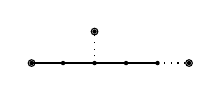
\begin{tikzpicture}[scale=0.4]
	\coordinate (1) at (0,0);
	\coordinate (A) at (1,0);
	\coordinate (B) at (2,0);
	\coordinate (C) at (3,0);
	\coordinate (D) at (4,0);
	\coordinate (2) at (5,0);
	\coordinate (3) at (2,1);
	
	\foreach \c in {1,2,3,A,B,C,D} {
		\fill (\c) circle (2pt);
	}
	\foreach \c in {1,2,3} {
		\draw (\c) circle (3pt);
	}

	\draw (1) -- (A);
	\draw (A) -- (B);
	\draw (B) -- (C);
	\draw (C) -- (D);
	\draw[dotted] (D) -- (2);
	\draw[dotted] (B) -- (3);
\end{tikzpicture}
\qquad
% LABEL 1235
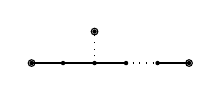
\begin{tikzpicture}[scale=0.4]
	\coordinate (1) at (0,0);
	\coordinate (A) at (1,0);
	\coordinate (B) at (2,0);
	\coordinate (C) at (3,0);
	\coordinate (D) at (4,0);
	\coordinate (2) at (5,0);
	\coordinate (3) at (2,1);
	
	\foreach \c in {1,2,3,A,B,C,D} {
		\fill (\c) circle (2pt);
	}
	\foreach \c in {1,2,3} {
		\draw (\c) circle (3pt);
	}

	\draw (1) -- (A);
	\draw (A) -- (B);
	\draw (B) -- (C);
	\draw[dotted] (C) -- (D);
	\draw (D) -- (2);
	\draw[dotted] (B) -- (3);
\end{tikzpicture}
\qquad
% LABEL 1245
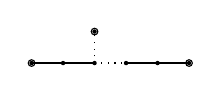
\begin{tikzpicture}[scale=0.4]
	\coordinate (1) at (0,0);
	\coordinate (A) at (1,0);
	\coordinate (B) at (2,0);
	\coordinate (C) at (3,0);
	\coordinate (D) at (4,0);
	\coordinate (2) at (5,0);
	\coordinate (3) at (2,1);
	
	\foreach \c in {1,2,3,A,B,C,D} {
		\fill (\c) circle (2pt);
	}
	\foreach \c in {1,2,3} {
		\draw (\c) circle (3pt);
	}

	\draw (1) -- (A);
	\draw (A) -- (B);
	\draw[dotted] (B) -- (C);
	\draw (C) -- (D);
	\draw (D) -- (2);
	\draw[dotted] (B) -- (3);
\end{tikzpicture}
\\[2em]
% LABEL 1345
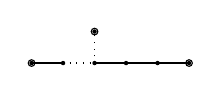
\begin{tikzpicture}[scale=0.4]
	\coordinate (1) at (0,0);
	\coordinate (A) at (1,0);
	\coordinate (B) at (2,0);
	\coordinate (C) at (3,0);
	\coordinate (D) at (4,0);
	\coordinate (2) at (5,0);
	\coordinate (3) at (2,1);
	
	\foreach \c in {1,2,3,A,B,C,D} {
		\fill (\c) circle (2pt);
	}
	\foreach \c in {1,2,3} {
		\draw (\c) circle (3pt);
	}

	\draw (1) -- (A);
	\draw[dotted] (A) -- (B);
	\draw (B) -- (C);
	\draw (C) -- (D);
	\draw (D) -- (2);
	\draw[dotted] (B) -- (3);
\end{tikzpicture}
\qquad
% LABEL 1346
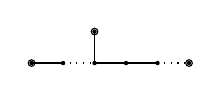
\begin{tikzpicture}[scale=0.4]
	\coordinate (1) at (0,0);
	\coordinate (A) at (1,0);
	\coordinate (B) at (2,0);
	\coordinate (C) at (3,0);
	\coordinate (D) at (4,0);
	\coordinate (2) at (5,0);
	\coordinate (3) at (2,1);
	
	\foreach \c in {1,2,3,A,B,C,D} {
		\fill (\c) circle (2pt);
	}
	\foreach \c in {1,2,3} {
		\draw (\c) circle (3pt);
	}

	\draw (1) -- (A);
	\draw[dotted] (A) -- (B);
	\draw (B) -- (C);
	\draw (C) -- (D);
	\draw[dotted] (D) -- (2);
	\draw (B) -- (3);
\end{tikzpicture}
\qquad
% LABEL 1356
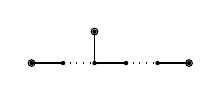
\begin{tikzpicture}[scale=0.4]
	\coordinate (1) at (0,0);
	\coordinate (A) at (1,0);
	\coordinate (B) at (2,0);
	\coordinate (C) at (3,0);
	\coordinate (D) at (4,0);
	\coordinate (2) at (5,0);
	\coordinate (3) at (2,1);
	
	\foreach \c in {1,2,3,A,B,C,D} {
		\fill (\c) circle (2pt);
	}
	\foreach \c in {1,2,3} {
		\draw (\c) circle (3pt);
	}

	\draw (1) -- (A);
	\draw[dotted] (A) -- (B);
	\draw (B) -- (C);
	\draw[dotted] (C) -- (D);
	\draw (D) -- (2);
	\draw (B) -- (3);
\end{tikzpicture}
\qquad
% LABEL 1456
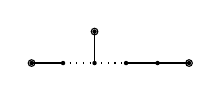
\begin{tikzpicture}[scale=0.4]
	\coordinate (1) at (0,0);
	\coordinate (A) at (1,0);
	\coordinate (B) at (2,0);
	\coordinate (C) at (3,0);
	\coordinate (D) at (4,0);
	\coordinate (2) at (5,0);
	\coordinate (3) at (2,1);
	
	\foreach \c in {1,2,3,A,B,C,D} {
		\fill (\c) circle (2pt);
	}
	\foreach \c in {1,2,3} {
		\draw (\c) circle (3pt);
	}

	\draw (1) -- (A);
	\draw[dotted] (A) -- (B);
	\draw[dotted] (B) -- (C);
	\draw (C) -- (D);
	\draw (D) -- (2);
	\draw (B) -- (3);
\end{tikzpicture}
\\[2em]
% LABEL 2345
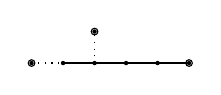
\begin{tikzpicture}[scale=0.4]
	\coordinate (1) at (0,0);
	\coordinate (A) at (1,0);
	\coordinate (B) at (2,0);
	\coordinate (C) at (3,0);
	\coordinate (D) at (4,0);
	\coordinate (2) at (5,0);
	\coordinate (3) at (2,1);
	
	\foreach \c in {1,2,3,A,B,C,D} {
		\fill (\c) circle (2pt);
	}
	\foreach \c in {1,2,3} {
		\draw (\c) circle (3pt);
	}

	\draw[dotted] (1) -- (A);
	\draw (A) -- (B);
	\draw (B) -- (C);
	\draw (C) -- (D);
	\draw (D) -- (2);
	\draw[dotted] (B) -- (3);
\end{tikzpicture}
\qquad
% LABEL 2346
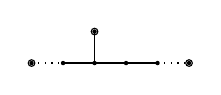
\begin{tikzpicture}[scale=0.4]
	\coordinate (1) at (0,0);
	\coordinate (A) at (1,0);
	\coordinate (B) at (2,0);
	\coordinate (C) at (3,0);
	\coordinate (D) at (4,0);
	\coordinate (2) at (5,0);
	\coordinate (3) at (2,1);
	
	\foreach \c in {1,2,3,A,B,C,D} {
		\fill (\c) circle (2pt);
	}
	\foreach \c in {1,2,3} {
		\draw (\c) circle (3pt);
	}

	\draw[dotted] (1) -- (A);
	\draw (A) -- (B);
	\draw (B) -- (C);
	\draw (C) -- (D);
	\draw[dotted] (D) -- (2);
	\draw (B) -- (3);
\end{tikzpicture}
\qquad
% LABEL 2356
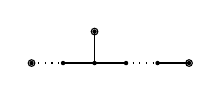
\begin{tikzpicture}[scale=0.4]
	\coordinate (1) at (0,0);
	\coordinate (A) at (1,0);
	\coordinate (B) at (2,0);
	\coordinate (C) at (3,0);
	\coordinate (D) at (4,0);
	\coordinate (2) at (5,0);
	\coordinate (3) at (2,1);
	
	\foreach \c in {1,2,3,A,B,C,D} {
		\fill (\c) circle (2pt);
	}
	\foreach \c in {1,2,3} {
		\draw (\c) circle (3pt);
	}

	\draw[dotted] (1) -- (A);
	\draw (A) -- (B);
	\draw (B) -- (C);
	\draw[dotted] (C) -- (D);
	\draw (D) -- (2);
	\draw (B) -- (3);
\end{tikzpicture}
\qquad
% LABEL 2456
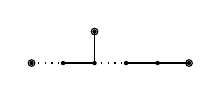
\begin{tikzpicture}[scale=0.4]
	\coordinate (1) at (0,0);
	\coordinate (A) at (1,0);
	\coordinate (B) at (2,0);
	\coordinate (C) at (3,0);
	\coordinate (D) at (4,0);
	\coordinate (2) at (5,0);
	\coordinate (3) at (2,1);
	
	\foreach \c in {1,2,3,A,B,C,D} {
		\fill (\c) circle (2pt);
	}
	\foreach \c in {1,2,3} {
		\draw (\c) circle (3pt);
	}

	\draw[dotted] (1) -- (A);
	\draw (A) -- (B);
	\draw[dotted] (B) -- (C);
	\draw (C) -- (D);
	\draw (D) -- (2);
	\draw (B) -- (3);
\end{tikzpicture}
\caption{Forests in $\trees(G;S)$.}
\label{fig:1-forests}
\end{figure}

\begin{figure}[h]
\centering
% LABEL 123
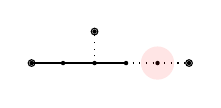
\begin{tikzpicture}[scale=0.4]
	\coordinate (1) at (0,0);
	\coordinate (A) at (1,0);
	\coordinate (B) at (2,0);
	\coordinate (C) at (3,0);
	\coordinate (D) at (4,0);
	\coordinate (2) at (5,0);
	\coordinate (3) at (2,1);
	
	\foreach \c in {1,2,3,A,B,C,D} {
		\fill (\c) circle (2pt);
	}
	\foreach \c in {1,2,3} {
		\draw (\c) circle (3pt);
	}

	\draw (1) -- (A);
	\draw (A) -- (B);
	\draw[dotted] (B) -- (3);
	\draw (B) -- (C);
	\draw[dotted] (C) -- (D);
	\draw[dotted] (D) -- (2);

	\draw[color=red, line width=12pt, cap=round, opacity=0.1] (D) -- (D);
\end{tikzpicture}
\qquad
% LABEL 124
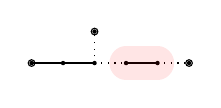
\begin{tikzpicture}[scale=0.4]
	\coordinate (1) at (0,0);
	\coordinate (A) at (1,0);
	\coordinate (B) at (2,0);
	\coordinate (C) at (3,0);
	\coordinate (D) at (4,0);
	\coordinate (2) at (5,0);
	\coordinate (3) at (2,1);
	
	\foreach \c in {1,2,3,A,B,C,D} {
		\fill (\c) circle (2pt);
	}
	\foreach \c in {1,2,3} {
		\draw (\c) circle (3pt);
	}

	\draw (1) -- (A);
	\draw (A) -- (B);
	\draw[dotted] (B) -- (3);
	\draw[dotted] (B) -- (C);
	\draw (C) -- (D);
	\draw[dotted] (D) -- (2);

	\draw[color=red, line width=12pt, cap=round, opacity=0.1] (C) -- (D);
\end{tikzpicture}
\qquad
% LABEL 125
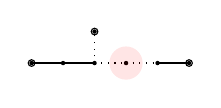
\begin{tikzpicture}[scale=0.4]
	\coordinate (1) at (0,0);
	\coordinate (A) at (1,0);
	\coordinate (B) at (2,0);
	\coordinate (C) at (3,0);
	\coordinate (D) at (4,0);
	\coordinate (2) at (5,0);
	\coordinate (3) at (2,1);
	
	\foreach \c in {1,2,3,A,B,C,D} {
		\fill (\c) circle (2pt);
	}
	\foreach \c in {1,2,3} {
		\draw (\c) circle (3pt);
	}

	\draw (1) -- (A);
	\draw (A) -- (B);
	\draw[dotted] (B) -- (3);
	\draw[dotted] (B) -- (C);
	\draw[dotted] (C) -- (D);
	\draw (D) -- (2);

	\draw[color=red, line width=12pt, cap=round, opacity=0.1] (C) -- (C);
\end{tikzpicture}
\\[2em]
% LABEL 134
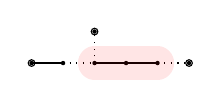
\begin{tikzpicture}[scale=0.4]
	\coordinate (1) at (0,0);
	\coordinate (A) at (1,0);
	\coordinate (B) at (2,0);
	\coordinate (C) at (3,0);
	\coordinate (D) at (4,0);
	\coordinate (2) at (5,0);
	\coordinate (3) at (2,1);
	
	\foreach \c in {1,2,3,A,B,C,D} {
		\fill (\c) circle (2pt);
	}
	\foreach \c in {1,2,3} {
		\draw (\c) circle (3pt);
	}

	\draw (1) -- (A);
	\draw[dotted] (A) -- (B);
	\draw[dotted] (B) -- (3);
	\draw (B) -- (C);
	\draw (C) -- (D);
	\draw[dotted] (D) -- (2);

	\draw[color=red, line width=12pt, cap=round, opacity=0.1] (B) -- (D);
\end{tikzpicture}
\qquad
% LABEL 135
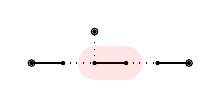
\begin{tikzpicture}[scale=0.4]
	\coordinate (1) at (0,0);
	\coordinate (A) at (1,0);
	\coordinate (B) at (2,0);
	\coordinate (C) at (3,0);
	\coordinate (D) at (4,0);
	\coordinate (2) at (5,0);
	\coordinate (3) at (2,1);
	
	\foreach \c in {1,2,3,A,B,C,D} {
		\fill (\c) circle (2pt);
	}
	\foreach \c in {1,2,3} {
		\draw (\c) circle (3pt);
	}

	\draw (1) -- (A);
	\draw[dotted] (A) -- (B);
	\draw[dotted] (B) -- (3);
	\draw (B) -- (C);
	\draw[dotted] (C) -- (D);
	\draw (D) -- (2);

	\draw[color=red, line width=12pt, cap=round, opacity=0.1] (B) -- (C);
\end{tikzpicture}
\qquad
% LABEL 136
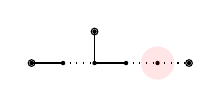
\begin{tikzpicture}[scale=0.4]
	\coordinate (1) at (0,0);
	\coordinate (A) at (1,0);
	\coordinate (B) at (2,0);
	\coordinate (C) at (3,0);
	\coordinate (D) at (4,0);
	\coordinate (2) at (5,0);
	\coordinate (3) at (2,1);
	
	\foreach \c in {1,2,3,A,B,C,D} {
		\fill (\c) circle (2pt);
	}
	\foreach \c in {1,2,3} {
		\draw (\c) circle (3pt);
	}

	\draw (1) -- (A);
	\draw[dotted] (A) -- (B);
	\draw (B) -- (3);
	\draw (B) -- (C);
	\draw[dotted] (C) -- (D);
	\draw[dotted] (D) -- (2);

	\draw[color=red, line width=12pt, cap=round, opacity=0.1] (D) -- (D);
\end{tikzpicture}
\qquad
% LABEL 145
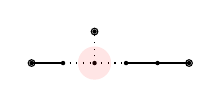
\begin{tikzpicture}[scale=0.4]
	\coordinate (1) at (0,0);
	\coordinate (A) at (1,0);
	\coordinate (B) at (2,0);
	\coordinate (C) at (3,0);
	\coordinate (D) at (4,0);
	\coordinate (2) at (5,0);
	\coordinate (3) at (2,1);
	
	\foreach \c in {1,2,3,A,B,C,D} {
		\fill (\c) circle (2pt);
	}
	\foreach \c in {1,2,3} {
		\draw (\c) circle (3pt);
	}

	\draw (1) -- (A);
	\draw[dotted] (A) -- (B);
	\draw[dotted] (B) -- (3);
	\draw[dotted] (B) -- (C);
	\draw (C) -- (D);
	\draw (D) -- (2);

	\draw[color=red, line width=12pt, cap=round, opacity=0.1] (B) -- (B);
\end{tikzpicture}
\\[2em]
% LABEL 146
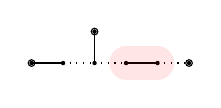
\begin{tikzpicture}[scale=0.4]
	\coordinate (1) at (0,0);
	\coordinate (A) at (1,0);
	\coordinate (B) at (2,0);
	\coordinate (C) at (3,0);
	\coordinate (D) at (4,0);
	\coordinate (2) at (5,0);
	\coordinate (3) at (2,1);
	
	\foreach \c in {1,2,3,A,B,C,D} {
		\fill (\c) circle (2pt);
	}
	\foreach \c in {1,2,3} {
		\draw (\c) circle (3pt);
	}

	\draw (1) -- (A);
	\draw[dotted] (A) -- (B);
	\draw (B) -- (3);
	\draw[dotted] (B) -- (C);
	\draw (C) -- (D);
	\draw[dotted] (D) -- (2);

	\draw[color=red, line width=12pt, cap=round, opacity=0.1] (C) -- (D);
\end{tikzpicture}
\qquad
% LABEL 156
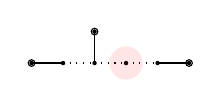
\begin{tikzpicture}[scale=0.4]
	\coordinate (1) at (0,0);
	\coordinate (A) at (1,0);
	\coordinate (B) at (2,0);
	\coordinate (C) at (3,0);
	\coordinate (D) at (4,0);
	\coordinate (2) at (5,0);
	\coordinate (3) at (2,1);
	
	\foreach \c in {1,2,3,A,B,C,D} {
		\fill (\c) circle (2pt);
	}
	\foreach \c in {1,2,3} {
		\draw (\c) circle (3pt);
	}

	\draw (1) -- (A);
	\draw[dotted] (A) -- (B);
	\draw (B) -- (3);
	\draw[dotted] (B) -- (C);
	\draw[dotted] (C) -- (D);
	\draw (D) -- (2);

	\draw[color=red, line width=12pt, cap=round, opacity=0.1] (C) -- (C);
\end{tikzpicture}
\qquad
% LABEL 234
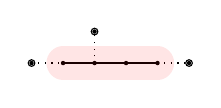
\begin{tikzpicture}[scale=0.4]
	\coordinate (1) at (0,0);
	\coordinate (A) at (1,0);
	\coordinate (B) at (2,0);
	\coordinate (C) at (3,0);
	\coordinate (D) at (4,0);
	\coordinate (2) at (5,0);
	\coordinate (3) at (2,1);
	
	\foreach \c in {1,2,3,A,B,C,D} {
		\fill (\c) circle (2pt);
	}
	\foreach \c in {1,2,3} {
		\draw (\c) circle (3pt);
	}

	\draw[dotted] (1) -- (A);
	\draw (A) -- (B);
	\draw[dotted] (B) -- (3);
	\draw (B) -- (C);
	\draw (C) -- (D);
	\draw[dotted] (D) -- (2);

	\draw[color=red, line width=12pt, cap=round, opacity=0.1] (A) -- (D);
\end{tikzpicture}
\qquad
% LABEL 235
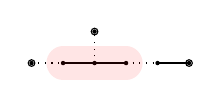
\begin{tikzpicture}[scale=0.4]
	\coordinate (1) at (0,0);
	\coordinate (A) at (1,0);
	\coordinate (B) at (2,0);
	\coordinate (C) at (3,0);
	\coordinate (D) at (4,0);
	\coordinate (2) at (5,0);
	\coordinate (3) at (2,1);
	
	\foreach \c in {1,2,3,A,B,C,D} {
		\fill (\c) circle (2pt);
	}
	\foreach \c in {1,2,3} {
		\draw (\c) circle (3pt);
	}

	\draw[dotted] (1) -- (A);
	\draw (A) -- (B);
	\draw[dotted] (B) -- (3);
	\draw (B) -- (C);
	\draw[dotted] (C) -- (D);
	\draw (D) -- (2);

	\draw[color=red, line width=12pt, cap=round, opacity=0.1] (A) -- (C);
\end{tikzpicture}
\\[2em]
% LABEL 236
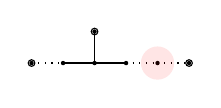
\begin{tikzpicture}[scale=0.4]
	\coordinate (1) at (0,0);
	\coordinate (A) at (1,0);
	\coordinate (B) at (2,0);
	\coordinate (C) at (3,0);
	\coordinate (D) at (4,0);
	\coordinate (2) at (5,0);
	\coordinate (3) at (2,1);
	
	\foreach \c in {1,2,3,A,B,C,D} {
		\fill (\c) circle (2pt);
	}
	\foreach \c in {1,2,3} {
		\draw (\c) circle (3pt);
	}

	\draw[dotted] (1) -- (A);
	\draw (A) -- (B);
	\draw (B) -- (3);
	\draw (B) -- (C);
	\draw[dotted] (C) -- (D);
	\draw[dotted] (D) -- (2);

	\draw[color=red, line width=12pt, cap=round, opacity=0.1] (D) -- (D);
\end{tikzpicture}
\qquad
% LABEL 245
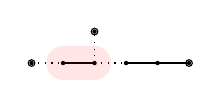
\begin{tikzpicture}[scale=0.4]
	\coordinate (1) at (0,0);
	\coordinate (A) at (1,0);
	\coordinate (B) at (2,0);
	\coordinate (C) at (3,0);
	\coordinate (D) at (4,0);
	\coordinate (2) at (5,0);
	\coordinate (3) at (2,1);
	
	\foreach \c in {1,2,3,A,B,C,D} {
		\fill (\c) circle (2pt);
	}
	\foreach \c in {1,2,3} {
		\draw (\c) circle (3pt);
	}

	\draw[dotted] (1) -- (A);
	\draw (A) -- (B);
	\draw[dotted] (B) -- (3);
	\draw[dotted] (B) -- (C);
	\draw (C) -- (D);
	\draw (D) -- (2);

	\draw[color=red, line width=12pt, cap=round, opacity=0.1] (A) -- (B);
\end{tikzpicture}
\qquad
% LABEL 246
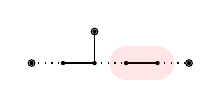
\begin{tikzpicture}[scale=0.4]
	\coordinate (1) at (0,0);
	\coordinate (A) at (1,0);
	\coordinate (B) at (2,0);
	\coordinate (C) at (3,0);
	\coordinate (D) at (4,0);
	\coordinate (2) at (5,0);
	\coordinate (3) at (2,1);
	
	\foreach \c in {1,2,3,A,B,C,D} {
		\fill (\c) circle (2pt);
	}
	\foreach \c in {1,2,3} {
		\draw (\c) circle (3pt);
	}

	\draw[dotted] (1) -- (A);
	\draw (A) -- (B);
	\draw (B) -- (3);
	\draw[dotted] (B) -- (C);
	\draw (C) -- (D);
	\draw[dotted] (D) -- (2);

	\draw[color=red, line width=12pt, cap=round, opacity=0.1] (C) -- (D);
\end{tikzpicture}
\qquad
% LABEL 256
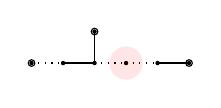
\begin{tikzpicture}[scale=0.4]
	\coordinate (1) at (0,0);
	\coordinate (A) at (1,0);
	\coordinate (B) at (2,0);
	\coordinate (C) at (3,0);
	\coordinate (D) at (4,0);
	\coordinate (2) at (5,0);
	\coordinate (3) at (2,1);
	
	\foreach \c in {1,2,3,A,B,C,D} {
		\fill (\c) circle (2pt);
	}
	\foreach \c in {1,2,3} {
		\draw (\c) circle (3pt);
	}

	\draw[dotted] (1) -- (A);
	\draw (A) -- (B);
	\draw (B) -- (3);
	\draw[dotted] (B) -- (C);
	\draw[dotted] (C) -- (D);
	\draw (D) -- (2);

	\draw[color=red, line width=12pt, cap=round, opacity=0.1] (C) -- (C);
\end{tikzpicture}
\\[2em]
% LABEL 345
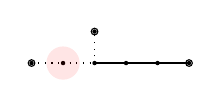
\begin{tikzpicture}[scale=0.4]
	\coordinate (1) at (0,0);
	\coordinate (A) at (1,0);
	\coordinate (B) at (2,0);
	\coordinate (C) at (3,0);
	\coordinate (D) at (4,0);
	\coordinate (2) at (5,0);
	\coordinate (3) at (2,1);
	
	\foreach \c in {1,2,3,A,B,C,D} {
		\fill (\c) circle (2pt);
	}
	\foreach \c in {1,2,3} {
		\draw (\c) circle (3pt);
	}

	\draw[dotted] (1) -- (A);
	\draw[dotted] (A) -- (B);
	\draw[dotted] (B) -- (3);
	\draw (B) -- (C);
	\draw (C) -- (D);
	\draw (D) -- (2);

	\draw[color=red, line width=12pt, cap=round, opacity=0.1] (A) -- (A);
\end{tikzpicture}
\qquad
% LABEL 346
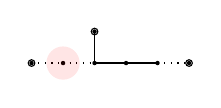
\begin{tikzpicture}[scale=0.4]
	\coordinate (1) at (0,0);
	\coordinate (A) at (1,0);
	\coordinate (B) at (2,0);
	\coordinate (C) at (3,0);
	\coordinate (D) at (4,0);
	\coordinate (2) at (5,0);
	\coordinate (3) at (2,1);
	
	\foreach \c in {1,2,3,A,B,C,D} {
		\fill (\c) circle (2pt);
	}
	\foreach \c in {1,2,3} {
		\draw (\c) circle (3pt);
	}

	\draw[dotted] (1) -- (A);
	\draw[dotted] (A) -- (B);
	\draw (B) -- (3);
	\draw (B) -- (C);
	\draw (C) -- (D);
	\draw[dotted] (D) -- (2);

	\draw[color=red, line width=12pt, cap=round, opacity=0.1] (A) -- (A);
\end{tikzpicture}
\qquad
% LABEL 356
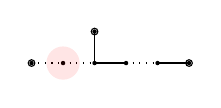
\begin{tikzpicture}[scale=0.4]
	\coordinate (1) at (0,0);
	\coordinate (A) at (1,0);
	\coordinate (B) at (2,0);
	\coordinate (C) at (3,0);
	\coordinate (D) at (4,0);
	\coordinate (2) at (5,0);
	\coordinate (3) at (2,1);
	
	\foreach \c in {1,2,3,A,B,C,D} {
		\fill (\c) circle (2pt);
	}
	\foreach \c in {1,2,3} {
		\draw (\c) circle (3pt);
	}

	\draw[dotted] (1) -- (A);
	\draw[dotted] (A) -- (B);
	\draw (B) -- (3);
	\draw (B) -- (C);
	\draw[dotted] (C) -- (D);
	\draw (D) -- (2);

	\draw[color=red, line width=12pt, cap=round, opacity=0.1] (A) -- (A);
\end{tikzpicture}
\qquad
% LABEL 456
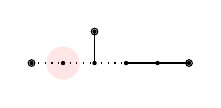
\begin{tikzpicture}[scale=0.4]
	\coordinate (1) at (0,0);
	\coordinate (A) at (1,0);
	\coordinate (B) at (2,0);
	\coordinate (C) at (3,0);
	\coordinate (D) at (4,0);
	\coordinate (2) at (5,0);
	\coordinate (3) at (2,1);
	
	\foreach \c in {1,2,3,A,B,C,D} {
		\fill (\c) circle (2pt);
	}
	\foreach \c in {1,2,3} {
		\draw (\c) circle (3pt);
	}

	\draw[dotted] (1) -- (A);
	\draw[dotted] (A) -- (B);
	\draw (B) -- (3);
	\draw[dotted] (B) -- (C);
	\draw (C) -- (D);
	\draw (D) -- (2);

	\draw[color=red, line width=12pt, cap=round, opacity=0.1] (A) -- (A);
\end{tikzpicture}
\caption{Forests in $\forests_2(G;S)$, with floating component highlighted.}
\label{fig:2-forests}
\end{figure}


\subsection{Laplacian matrix}

Given a graph $G = (V,E)$, let $L \in \RR^{V \times V}$ denote the {\em Laplacian matrix} of $G$.
If $G$ is a weighted graph with edge weights $\alpha_e  \in \RR_{>0}$ for $e \in E$,
let $L$ denote the weighted Laplacian matrix of $G$.

\begin{dfn}[Weighted Laplacian matrix]
Given a graph $G = (V,E)$ and edge weights $\{ \alpha_e : e \in E\}$,
the {\em weighted Laplacian matrix} $\La \in \RR^{V\times V}$ is defined by
\[
	(\La)_{v,w} = \begin{cases}
		0 &\text{if } v\neq w \text{ and } (v,w) \not\in E \\
		- \alpha_e^{-1} &\text{if } v\neq w \text{ and } (v,w) = e \in E \\
		\displaystyle \sum_{e \in N(v)} \alpha_e^{-1} &\text{if } v = w.
	\end{cases}
\]
\end{dfn}

Given $S \subset V$,
let $L[\overline S]$ denote the matrix obtained from $L$ by removing the rows and columns indexed by $S$.
For any graph $G$, let $\kappa(G)$ denote the number of spanning trees of $G$.
The following theorem related minors of the (weighted) Laplacian to (weighted) counts of rooted spanning forests.
%is due to Kirchhoff.
\begin{thm}[Principal-minors matrix tree theorem]
\label{thm:matrix-tree}
Let $G = (V,E)$ be a finite graph.
\begin{enumerate}[(a)]
\item 
Let $L$ denote the Laplacian matrix of $G$.
Then for any nonempty vertex set $S \subset V$,
\begin{equation}
	\det L[\overline S] = \kappa( G ; S) .
\end{equation}

\item 
Let $L_\alpha$ denote the weighted Laplacian matrix of $G$, with edge weights $\{\alpha_e\}$. 
Then for any nonempty vertex set $S \subset V$,
\begin{equation}
	\det L_\alpha[\overline S] = \sum_{T \in \trees( G ; S)} w(T)^{-1}
	= \sum_{T \in \trees(G; S)} w(\overline{T}) \prod_{e \in E} \alpha_e^{-1} .
\end{equation}
\end{enumerate}
\end{thm}
\begin{proof}
See Tutte~\cite[Section VI.6, Equation (VI.6.7)]{tutte} or Chaiken~\cite{chaiken} or Bapat~\cite[Theorem 4.7]{bapat}.
\end{proof}

Note that $\kappa(G;S)$ is also the number of 
% $S$-rooted spanning forests of $G$.
spanning trees of the quotient graph $G / S$, which ``glues together'' all vertices in $S$ as a single vertex.

Next we recall a connection between minors of the Laplacian matrix and cofactor sums of the distance matrix, when $G$ is a tree.
The result is due to Bapat--Sivasubramanian~\cite{bapat-sivasubramanian}.
Recall that $\cof M$ denotes the {\em sum of cofactors} of $M$, i.e. 
$\displaystyle
	\cof M = \sum_{i = 1}^{n} \sum_{j = 1}^{n} (-1)^{i + j} \det M[\overline{i},\overline{j}].
$

\begin{thm}[Distance submatrix cofactor sums]
\label{thm:distance-sub-cof}
Given a tree $G$ with edge weights,
let $D$ be the weighted distance matrix of $G$, and $L$ the weighted Laplacian matrix of $G$.
Let $S \subset V(G)$ be a nonempty subset of vertices of $G$. 
Then
\begin{equation}
	\cof D[S] = (-2)^{|S|-1} \sum_{T \in \trees(G; S)} w(\overline{T}).
\end{equation}
\end{thm}
\begin{proof}
Bapat and Sivasubramanian~\cite[Theorem 11]{bapat-sivasubramanian}
show that
\[
	\cof D[S] = (-2)^{|S|-1} \left( \prod_{e \in E} \alpha_e \right) \det L[\overline S] .
\]
Then combine this equation with the matrix tree theorem,
Theorem~\ref{thm:matrix-tree} (b).
\end{proof}

% \subsection{Distance in trees}
\subsection{Tree splits and tree distance}
\label{sec:tree-splits}

In this section we describe the tree splits associated to a tree, and use their associated indicator functions to give an expression for the tree distance.

Given a tree $G = (V,E)$ and an edge $e \in E$, the edge deletion $G \setminus e$ contains two connected components.
Using the implicit orientation on $e = (e^+,e^-)$,
we let $(G \setminus e)^+$ denote the component that contains endpoint $e^+$, and let $(G\setminus e)^-$ denote the other component.
For any $e \in E$ and $v \in V$,
we let
$(G \setminus e)^{v}$ denote the component of $G\setminus e$ containing $v$,
respectively $(G\setminus e)^{\overline v}$ for the component not containing $v$.

%\subsection{Tree distance}
%\label{sec:tree-distance}

Tree splits can be used to express the path distance between vertices in a tree.
Given an edge $e\in E$ and vertices $v,w \in V$, let 
\begin{equation}
\delta(e;v,w) = \begin{cases}
	1 &\text{if $e$ separates  $v$ from $w$}, \\
	%1 &\text{if $e$ lies on $v\sim w$ path}, \\
	0 &\text{otherwise}.
\end{cases}
\end{equation}
In other words, $\delta(e; v,w) = 1$ if the vertices are in different components of the split $G \setminus e$,
and $\delta(e; v,w) = 0$ if they are in the same component.
Note that $\delta(e; v,v) = 0$ for any $e$ and $v$.
%\begin{equation}
%\delta(e; v,w) = \begin{cases}
%1 &\text{if $e$ lies on $v\sim w$ path}, \\
%0 &\text{otherwise}.
%\end{cases}
%\end{equation}

We have the following perspectives on the function $\delta(e; v,w)$:
\begin{enumerate}[(i)]
\item 
If we fix $e$ and $v$,
then $\delta(e;v, -) : V(G) \to \{0,1\}$ 
is the indicator function for the component 
$(G \setminus e)^{\overline v}$ of the tree split $G \setminus e$
%of $G \setminus e$ 
not containing $v$.

\item 
On the other hand if we fix $v$ and $w$, then $\delta(-;v,w) : E(G) \to \{0,1\}$
is the indicator function for the unique $v \sim w$ path in $G$.

\end{enumerate}


\begin{prop}[Weighted tree distance]
\label{prop:distance-sum}
For a tree $G = (V,E)$ with weights $\{\alpha_e : e \in E\}$,
the weighted distance function satisfies
\[ d_\alpha(v,w) = \sum_{e \in E} \alpha_e \, \delta(e; v,w) .\]
\end{prop}

For an unweighted tree, we can express the tree distance $d(v,w)$ as the unweighted sum
\begin{equation*}
	d(v,w) = \sum_{e \in E(G)} \delta(e; v,w).
\end{equation*}


\subsection{Outdegree of rooted forest}

Given a vertex $v$ in a graph, the {\em degree} $\deg(v)$ is the number of edges incident to $v$.
%The ``handshake lemma'' of graph theory states that  $\sum_{v \in V(G)} \deg(v) = 2|E|$.
A consequence of the ``handshake lemma'' of graph theory is that for any tree $G$, we have
\[
\sum_{v \in V(G)} (2 - \deg(v)) = 2.
\]
In this section we discuss some generalizations, which will be used later.

Given a connected subgraph $H \subset G$,
we define the {\em outdegree} $\degout(H)$ as the number of edges which join $H$ to its complement; i.e.
\begin{equation}
	\degout(H) = \#\{ e = (a,b) \in E : a \in V(H),\, b \not\in V(H)\}.
\end{equation}

\begin{lem}
\label{lem:outdeg-sum}
Suppose $G$ is a tree.
\begin{enumerate}[(a)]
\item 
If $H\subset G$ is a (nonempty) connected subgraph, then
\[
  \sum_{v \in V(H)} \left( 2 -  \deg(v) \right) = 2 - \degout(H) .
\]

\item 
If $e$ is a fixed edge and $u$ is a fixed vertex of $G$, then
\[
	\sum_{v \in V(G)} (2 - \deg(v)) \delta(e; u,v) = 1.
\]

\end{enumerate}
\end{lem}
\begin{proof}
(a)
This is straightforward to check by induction on $|V(H)|$,
with base case $|V(H)| = 1$:
if $H = \{v\}$ consists of a single vertex, then $\degout(H) = \deg(v)$.
%
%Now consider $|V(H)| = n > 1$, and suppose the claim is true for $H'$ when $|V(H')| < n$.
%Since $H$ is a subgraph of a tree, it contains a vertex $v_0$ whose $H$-degree is one.
%Let $H_0 = H \setminus v_0$.
%Using the induction hypothesis, we have
%\begin{align}
% \sum_{v \in V(H)} 2 - \deg(v) &= 2 - \deg(v_0) + \sum_{v \in V(H_0)} 2 - \deg(v) \\
% &= 2 - \deg(v_0) + 2 - \degout(H_0) \\
% &= 2 - \left( \degout(H_0) + \deg(v_0) - 2 \right) .
%\end{align}
%Thus it suffices to show that
%\[ 
%  \degout(H) = \degout(H_0) + \deg(v_0) - 2.
%\]
%This hold because $\degout(H_0) + \deg(v_0)$ overcounts the unique edge joining $v_0$ to $H_0$, by two.

(b)
Using part (a), we have
\[
	\sum_{v \in V} (2 - \deg(v)) \delta(e; u,v)
	= \sum_{v \in (G \setminus e)^{\overline u}} (2 - \deg(v))
	= 2 - \degout((G \setminus e)^{\overline u}) = 1. 
\] 
Since the component $(G \setminus e)^{\overline u}$ of the tree split $G \setminus e$ has a single edge separating it from its complement, 
$\degout((G \setminus e)^{\overline u}) = 1$
\end{proof}

OLD: Given a rooted forest $F$ in $\forests_1(G;S)$ and $s \in S$,
let $F(s)$ denote the $s$-component of $F$.
We define the {\em outdegree} $\degout(F,s)$ as the number of edges which join $F(s)$ to a different component; i.e.
\begin{equation}
\label{eq:outdeg}
	\degout(F,s) = \#\{ e = (a,b) \in E : a \in F(s),\, b \not\in F(s)\}.
\end{equation}
%In words, $\degout(F,s)$ is the number of edges which connect the $s$-component of $F$ to a different component.
%\[
%	\#\{ e \in E : e \text{ connects the $s$-component of $F$ to a different component}\}
%\]
If $F$ is a forest in $\forests_2(G;S)$, let $\degout(F,*)$ denote the outdegree of the floating component.

\subsection{Miscellaneous}

Later we will make use of the fact that a submatrix $D[S]$ of a distance matrix has nonzero determinant, as long as $|S| \geq 2$.

We first recall a result of Cauchy, which states that the eigenvalues of $M[\overline{i}]$ ``interlace'' the eigenvalues of $M$.
Recall that $M[\overline{i}]$ denotes the matrix obtained from $M$ by deleting the $i$-th row and column.

\begin{prop}[Cauchy interlacing]
\label{prop:cauchy-interlacing}
Suppose $M$ is a symmetric real matrix 
with ordered eigenvalues $\lambda_1 \leq \cdots \leq \lambda_n$, 
and  the submatrix $M[\overline{i}]$ has ordered eigenvalues $\mu_1 \leq \cdots \leq \mu_{n-1}$.
Then
\[
	\lambda_1 \leq \mu_1 \leq \lambda_2 \leq \cdots \leq \mu_{n-1} \leq \lambda_n.
\]
\end{prop}
\begin{proof}
See Horn--Johnson~\cite[Theorem 4.3.17]{horn-johnson}.
\end{proof}

\begin{lem}[{Bapat~\cite[Lemma 8.15]{bapat}}]
\label{lem:dist-signature}
Suppose $D$ is the (weighted) distance matrix of a tree with $n$ vertices. 
Then $D$ has one positive eigenvalue and $n - 1$ negative eigenvalues.
\end{lem}
\begin{proof}
Lemma 8.15 of~\cite{bapat} is stated for a non-weighted distance matrix;
however, the same argument applies to a weighted distance matrix by applying Bapat--Kirkland--Neumann's result \eqref{eq:w-full-det} on the weighted distance matrix determinant \cite[Corollary 2.5]{bapat-kirkland-neumann}. 
\end{proof}

The following argument was communicated to the author by Bapat, via personal communication.
\begin{prop}
\label{prop:distance-sub-nonsingular}
Suppose $D$ is the distance matrix of a tree $G = (V,E)$ and $S \subset V$ is a subset of size $|S| \geq 2$. 
Then
\begin{enumerate}[(a)]
\item $D[S]$ has one positive eigenvalue and $|S| - 1$ negative eigenvalues;

\item $\det D[S] \neq 0$.

\end{enumerate}
\end{prop}
\begin{proof}
(a) Let $n = |V|$; assume $n \geq 3$.
We apply (decreasing) induction on the size of $S$. 
If $|S| = n - 1$, then Lemma~\ref{lem:dist-signature} and Cauchy interlacing imply that $D[S]$ has at most one positive eigenvalue, and at least one negative eigenvalue. 
Since all diagonal entries of $D[S]$ are zero, $D[S]$ has zero trace. 
Thus $D[S]$ has exactly one positive eigenvalue as claimed.
The same argument applies for smaller $S$, as long as $|S| \geq 2$.

(b) This follows from (a), since the determinant is the product of eigenvalues.
\end{proof}


\begin{rmk}
A key step in the main proof is the use of the map
\[
	E(G) \times \trees(G;S) \mapsto S \sqcup \{\text{error}\}
\]
defined by
\[
	(e, T) \mapsto \begin{cases}
		s &\text{if } e \in T(s), \\
		\text{error} &\text{if } e \not\in T .
	\end{cases}
\]
\end{rmk}

\begin{rmk}
For a given spanning forest
$F \in \forests_2(G;S)$,
there are exactly $\degout(F, *)$-many choices of pairs $(T,e) \in \trees(G;S) \times E(G)$ such that
$F = T \setminus e.$
Consider the ``deletion'' map
\[
	E(G) \times \trees(G;S) \to \forests_2(G;S) \sqcup \trees(G;S)
\]
defined by
\[
	(e, T) \mapsto \begin{cases}
	T \setminus e &\text{if } e\in T,\\
	T &\text{if } e\not\in T.
	\end{cases}
\]
For a forest $F$ in $\forests_2(G;S)$,
the preimage under this map has $\degout(F,*)$ elements.

There is an associated ``union'' map 
\[
	E(G) \times \forests_2(G;S) \longrightarrow \trees(G;S) \sqcup \forests_2(G;S)
\]
defined by
\[
	(e, F) \mapsto \begin{cases}
		F \cup e &\text{if } e \in \partial F, \\
		F &\text{if } e \not\in \partial F
	\end{cases}
\]
For a forest $T$ in $\trees(G; S)$, the preimage under this map has $|E(T)|$-many elements.
\end{rmk}


\section{Optimization: quadratic programming}
\label{sec:optimization}

\begin{prop}
If $D[S]$ is a principal submatrix of a distance matrix indexed by $S$, then 
%any critical value of the optimization problem \note{cite above} is equal to ${\det D[S]}/{\cof D[S]}$, i.e.
\[
	\frac{\det D[S]}{\cof D[S]} = \max \{\boldm^\tr D[S] \boldm : \boldm \in \RR^S,\, \bone^\tr \boldm = 1 \}
\]
where $\cof D[S]$ denotes the sum of cofactors of $D[S]$.
\end{prop}

\begin{prop}
If $D[S]$ is a principal submatrix of a distance matrix indexed by $S$, then 
\[
	\frac{\det D[S]}{\cof D[S]} = \max \{\boldm^\tr D \boldm : \boldm \in \RR^V,\, \bone^\tr \boldm = 1,\, \boldm_v = 0 \text{ if } v \not\in S \}
\]
where $\cof D[S]$ denotes the sum of cofactors of $D[S]$.
\end{prop}
\begin{proof}
The gradient of the objective function is $2 D[S] \boldm$, 
and the gradient of the constraint is $\bone$.
By the theory of Lagrange multipliers, the optimal solution $\boldm^*$ is a vector satisfying
\[
	D[S] \boldm^* = \lambda \bone \qquad\text{for some }\lambda \in \RR.
\]
The constant $\lambda$ is in fact the optimal objective value, since
\[
	(\boldm^*)^\tr D[S] \boldm^* = (D[S] \boldm^*)^\tr \boldm^* = \lambda (\bone^\tr \boldm^*) = \lambda.
\]
The above computation uses the fact that $D[S]$ is a symmetric matrix, and the given constraint $\bone^\tr \boldm = 1$.

On the other hand,
assuming $D[S]$ is invertible we have $ \boldm^* = \lambda (D[S]^{-1} \bone) $, so that
\[
	1 = \bone^\tr \boldm^* = \lambda (\bone^\tr D[S]^{-1} \bone)
	= \lambda \frac{\cof D[S]}{\det D[S]}.
\]
Thus the optimal objective value is
$\displaystyle
	\lambda = \frac{\det D[S]}{\cof D[S]} .
$
\end{proof}

\section{Distance submatrices: Proofs}
In this section we prove our main result, Theorem~\ref{thm:w-main}.
Theorem~\ref{thm:main} follows as an immediate corollary.
% by setting all edge weights to one.

Outline of proof: given a  subset $S \subset V$ and distance submatrix $D[S]$, we will
\begin{enumerate}[(i)]
\item 
Find vector $\boldm \in \RR^S$ such that $D[S]\boldm = \lambda \mathbf{1} \in \RR^S$.

\item 
Compute the sum of entries of $\boldm$, i.e. $\mathbf{1}^\tr \boldm$.

\item 
Using (i), relate the sum $\bone^\tr \boldm$ to the sum of entries of the inverse matrix $D[S]^{-1}$:
%note the identity
$$ \mathbf{1}^\tr \boldm 
= \lambda (\mathbf{1}^\tr D[S]^{-1} \mathbf{1}) 
= \lambda \frac{\cof D[S]}{\det D[S]} .$$
where $\cof D[S]$ is the sum of cofactors of $D[S]$.

\item 
Use known expression for $\cof D[S]$ to compute
$$
\det D[S] = \lambda (\cof D[S]) \left( \mathbf{1}^\tr \boldm \right)^{-1}.
$$
\end{enumerate}
The interesting part  of this expression will turn out to be in the constant $\lambda$.

\begin{eg}
Suppose $G$ is a tree consisting of three paths joined at a central vertex.
Let $S$ consist of the central vertex, and the three endpoints of the paths. 
The corresponding submatrix of the distance matrix is
$$
D[S] = \begin{bmatrix}
0 & a & b & c \\
a & 0 & a + b & a + c \\
b & a + b & 0 & b + c \\
c & a + c & b + c & 0
\end{bmatrix}.
$$
Following the steps outlined above:
\begin{enumerate}[(i)]
\item 
The vector $\boldm = \begin{bmatrix} -1 \\ 1 \\ 1 \\ 1 \end{bmatrix}$ satisfies
$
D[S] \boldm = (a+b+c) \mathbf{1}
$

\item 
The sum of entries of $\boldm$ is $\mathbf{1}^\tr \boldm = 2$.

\item 
We have 
$$2 = \mathbf{1}^\tr \boldm = \lambda (\mathbf{1}^\tr D[S]^{-1} \mathbf{1}) = \displaystyle \lambda \frac{\cof D[S]}{\det D[S]}.$$

\item 
The cofactor sum  
$\cof D[S]$ is $-8 abc$,
so the determinant is
\begin{align*}
\det D[S] 
= \lambda \frac{\cof A}{\mathbf{1}^\tr \boldm}
= (a+b+c) (-8 abc)\frac{1}{2}
= -4(a+b+c)abc.
\end{align*}
\end{enumerate}
\end{eg}

\subsection{Warmup case: $S = V$}

\begin{prop}
Let $G = (V,E)$ a tree, and consider the vector $\boldm \in \RR^V$
defined by 
\begin{equation}
\boldm_v = 2 - \deg v
\qquad\text{for each }v\in V.
\end{equation}
% where $\deg v$ denotes the degree of $v$ in $G$.
Then $\mathbf{1}^\tr \boldm = \sum_{v \in V} (2-\deg v) = 2$.
\end{prop}
\begin{proof}
For any graph, $\sum_{v\in V} \deg v = 2 |E|$.
Since $G$ is a tree, $|E| = |V|-1$.
\end{proof}

\begin{prop}
\label{prop:m-distance-warmup}
Let $\boldm$ be the vector defined above,
and let $D$ be the distance matrix of $G$.
Then $D \boldm = \lambda \bone$
for some constant $\lambda$.
\end{prop}
\begin{proof}
%The distance matrix has entries $D_{v,w} = d(v,w)$ which can be expressed as
%\[
%d(v,w) = \sum_{e \in E} \alpha_e \delta(e;v,w),
%\]
%where $\delta(e;v,w)$ is defined in \note{cite}.

%Then for any $w \in V$,
%\begin{align}
%(D \boldm)_w &= \sum_{v \in V} d(v,w) (2 - \deg v) \\
%&= \sum_{v\in V} \left(\sum_{e \in E} \alpha_e \delta(e;v,w)\right) (2 - \deg v) \\
%&= \sum_{e\in E} \alpha_e \left(\sum_{v\in V} \delta(e;v,w) (2 - \deg v) \right) \\
%&= \sum_{e\in E} \alpha_e \sum_{v \in (G\setminus e)^{-w}} (2 - \deg v) \\
%&= \sum_{e\in E} \alpha_e ( 2 - \degout (G\setminus e)^{-w})
%\end{align}
%\note{improve: skip some above details}
It suffices to show that for each edge $e$, with endpoints $(e^+,e^-)$, we have
\[ 
	(D \boldm)_{(e^+)} = (D \boldm)_{(e^-)} .
\]
We compute
\begin{align}
	(D \boldm)_{(e^+)} - (D \boldm)_{(e^-)} &= \sum_{v \in V} (d(v,e^+) - d(v,e^-)) (2 - \deg v) \\
	&= \sum_{v\in (G\setminus e)^-}  \alpha_e (2 - \deg v)  - \sum_{v\in (G\setminus e)^+} \alpha_e (2 - \deg v) \\
	&= \alpha_e \left( \sum_{v\in (G\setminus e)^-}  (2 - \deg v)  - \sum_{v\in (G\setminus e)^+} (2 - \deg v)\right) 
\label{eq:12-1}
\end{align}
since
\[
	d(v,e^+) - d(v,e^-) = \begin{cases}
	\alpha_e &\text{if $v$ is closer to $e^-$ than }e^+,\\
	- \alpha_e &\text{if $v$ is closer to $e^+$ than }e^-.
	\end{cases}
\]
For each sum in \eqref{eq:12-1}, we apply Lemma~\ref{lem:outdeg-sum} to obtain
\begin{align}
\sum_{v \in (G\setminus e)^-}  (2 - \deg v) &= (2 - \degout( (G\setminus e)^-) 
= 1 ,
\end{align}
since each component of $(G \setminus e)$ has outdegree one.
The same identity applies to the sum over $(G \setminus e)^+$, so $(D\boldm)_{(e^+)} = (D\boldm)_{(e^-)}$ as desired.
\end{proof}

\subsection{General case: $S \subset V$}
Fix a tree $G = (V,E)$ and a nonempty subset $S \subset V$.
\begin{dfn}
\label{dfn:m-vector}
Let $\boldm = \boldm(G;S)$ denote the vector in $\RR^S$ be defined by
\begin{equation}
\label{eq:m-vector}
\boldm_v =  \sum_{T \in \trees(G;S)} (2 - \degout(T,v)) w(\overline{T})
\qquad\text{for each }v \in S.
\end{equation}
where $\degout(T,v)$ is the outdegree of the $v$-component of $T$, \eqref{eq:outdeg}.
\end{dfn}

Let $\bone$ denote the all-ones vector.
\begin{prop}
\label{prop:m-sum}
For the vector $\boldm$ defined above, 
\begin{enumerate}[(a)]
\item 
$\displaystyle \bone^\tr \boldm = 2 \,\sum_{T \in \trees(G;S)} w(\overline{T})$;

\item 
if all edge weights $\alpha_e$ are positive, $\boldm$ is nonzero.
\end{enumerate}
\end{prop}
\begin{proof}
(a)
By Lemma~\ref{lem:outdeg-sum} we have
\[
\boldm_s = \sum_{T \in \trees(G;S)} w(\overline{T}) (2 - \degout (T,s))
= \sum_{T \in \trees(G;S)} w(\overline{T}) \left( \sum_{v \in T(s)}(2 - \deg(v))\right).
\]
Then exchange the order of summation in $\bone^\tr \boldm$,
\begin{align}
	\bone^\tr \boldm = \sum_{s\in S} \boldm_s &= \sum_{s \in S} \left( \sum_{T \in \trees(G;S)} w(\overline{T}) \sum_{v \in T(s)}(2 - \deg(v)) \right) \\
	&= \sum_{T \in \trees(G;S)} w(\overline{T}) \left( \sum_{s\in S} \sum_{v \in T(s)} (2 - \deg(v)) \right) .
\end{align}
Next observe that the inner double sum is simply a sum over $v \in V$,
since the vertex sets of $T(s)$ for $s \in S$ form a partition of $V$ by definition of $S$-rooted spanning forest.
Thus 
\[
	\bone^\tr \boldm = \sum_{T \in \trees} w(\overline{T}) \left( \sum_{v \in V} (2 - \deg(v))\right)
	= \sum_{T \in \trees} w(\overline{T}) \cdot 2 
\]
where we again apply Lemma~\ref{lem:outdeg-sum} for the last equality, as $\degout(G) = 0$.

(b) 
If all edge weights are positive, then $w(\overline{T}) > 0$ for all $T$, and $\trees(G; S)$ is nonempty as long as $S$ is nonempty. 
Thus part (a) implies that $\bone^\tr \boldm > 0$.
\end{proof}

\begin{cor}
If $G$ is a graph with unit edge weights $\alpha_e = 1$, then the vector $\boldm$ defined in \eqref{eq:m-vector} satisfies $\bone^\tr \boldm = 2\, \kappa(G;S)$.
\end{cor}

\begin{thm}
\label{thm:m-distance-product}
With $\boldm = \boldm(G;S)$ defined as in \eqref{eq:m-vector},
$D[S] \boldm = \lambda \mathbf{1}$
for the constant
\begin{equation}
\label{eq:lambda}
	\lambda = \sum_{E(G)} \alpha_e \sum_{\trees(G;S)} w(\overline{T}) - \sum_{\forests_2(G;S)} (2 - \degout(F,*) )^2 \, w(\overline{F}) .
\end{equation}
%where $\degout(F,w)$ is the out-degree of the $w$-component of $F$ (as a spanning forest).
\end{thm}

\begin{proof}
For $e\in E$ and $v,w\in V$, let $\delta(e;v,w)$ denote the function defined in Section~\ref{sec:tree-splits}.
%\[
%  \delta(e;v,w) = \begin{cases}
%  1 &\text{if $e$ separates  $v$ from $w$}, \\
%  0 &\text{otherwise}.
%  \end{cases}
%\]
For any $v \in S$, we have
\begin{align}
  (D[S] \boldm)_v &= \sum_{s \in S} d(v,s) \boldm_s \\
  &= \sum_{s \in S} \left( \sum_{e \in E(G)} \alpha_e\, \delta(e; v,s) \right) \left( \sum_{T \in \trees(G;S)} (2 - \degout(T,s)) w(\overline{T}) \right) \\
  &= \sum_{T\in \trees} w(\overline{T}) \sum_{e\in E} \alpha_e \left( \sum_{s \in S} \delta(e; v,s) (2 - \deg^o(T, s)) \right) \\
  % &= \sum_{T \in \trees} w(\overline{T}) \sum_{e \in E} \alpha_e \left( \sum_{s \in S \cap (G\setminus e)^{\overline v}} (2 - \deg^o(T, s)) \right) \\
  &= \sum_{T \in \trees} w(\overline{T}) \sum_{e \in E} \alpha_e \left( \sum_{s \in S} \delta(e; v,s) \sum_{u \in T(s)} (2 - \deg(u)) \right). \label{eq:14-1}
\end{align}
%where
%\[ 
%	S \cap (G\setminus e)^{\overline v} = \{ s \in S : \text{$e$ separates $v$ from $s$}\}.
%S^*(e,v) = \{ s \in S : \text{$e$ lies on path from $v$ to $s$}\}.
%\]
where in the last equality, we apply Lemma~\ref{lem:outdeg-sum} to the subgraph $H = T(s)$.

We introduce additional notation to handle the double sum in parentheses in \eqref{eq:14-1}.
Each $S$-rooted spanning tree $T$ naturally induces a surjection $\pi_T: V \to S$, defined by 
\[
	\pi_T(u) = s \qquad\text{if and only if}\qquad u \in T(s).
\]
Using this notation,
\begin{equation}
\label{eq:9}
	(D[S] \boldm)_v = \sum_{T \in \trees} w(\overline{T}) \sum_{e \in E} \alpha_e \left( \sum_{u \in V} (2 - \deg(u)) \delta(e; v,\pi_T(u)) \right)
\end{equation}
We will compare the above expression with the one obtained after replacing $\delta(e; v,\pi_T(u))$ with $\delta(e; v, u)$.
From Lemma~\ref{lem:outdeg-sum} again, for any $v \in V$ and $e \in E$ we have
\[
	\sum_{u \in V} (2 - \deg(u)) \delta(e; v,u)
	= \sum_{u \in (G \setminus e)^{\overline v}} (2 - \deg(u))
	= 2 - \degout((G \setminus e)^{\overline v}) = 1. 
\] 
Thus
\begin{equation}
\label{eq:10}
	\sum_{T \in \trees} w(\overline{T}) \sum_{e \in E} \alpha_e
	= \sum_{T \in \trees} w(\overline{T}) \sum_{e \in E} \alpha_e \left( \sum_{u \in V} (2 - \deg(u)) \delta(e; v,u) \right) 
\end{equation}
After subtracting equation \eqref{eq:10} from \eqref{eq:9},
\[
	(D[S] \boldm)_v - \sum_{T \in \trees} w(\overline{T}) \sum_{e \in E} \alpha_e = \sum_{T \in \trees} w(\overline{T}) \sum_{e \in E} \alpha_e \sum_{u \in V} (2 - \deg(u)) \Big(\delta(e; v, \pi_T(u)) - \delta(e; v, u) \Big)
\]
When $e \in E$ and $v \in V$ are fixed, $u \mapsto \delta(e; v, u)$ is the indicator function of one component of the principal cut $G \setminus e$.
%Recall that $\delta(e; \cdot,\cdot)$ is a $(0,1)$-valued pseudometric on $V$.
We have
\begin{equation}
\label{eq:delta-diff}
	\delta(e; v, \pi_T(u)) - \delta(e; v, u) = \begin{cases}
	0 &\text{if } \delta(e; \pi_T(u), u) = 0 \\
	1 &\text{if } \delta(e; \pi_T(u), u) = 1 \text{ and } \delta(e; v, \pi_T(u)) = 1 \\
	-1 &\text{if } \delta(e; \pi_T(u), u) = 1 \text{ and } \delta(e; v, \pi_T(u)) = 0
	\end{cases}
\end{equation}
Now consider varying $u$ over all vertices, when $e$, $T$, and $v$ are fixed.
We have the following three cases:

Case 1: if $e \not \in T$, then $u$ and $\pi_T(u)$ are on the same side of the principal cut $G \setminus e$, for every vertex $u$.
In this case $\delta(e;v, \pi_T(\cdot)) - \delta(e; v, \cdot) = 0$.

Case 2: if $e \in T(s_0)$ and $s_0$ is separated from $v$ by $e$, then $\delta(e;v, \pi_T(\cdot)) - \delta(e; v, \cdot)$ is the indicator function for the floating component of $T \setminus e$. See Figure~\ref{fig:e-delete-from-forest}, left.

Case 3: if $e \in T(s_0)$ and $s_0$ is on the same component as $v$ from $e$, then $\delta(e;v, \pi_T(\cdot)) - \delta(e; v, \cdot)$ is the negative of the indicator function for the floating component of $T \setminus e$. See Figure~\ref{fig:e-delete-from-forest}, right.

\begin{figure}[h]
\begin{minipage}{0.45\textwidth}
\centering
% LABEL 2356
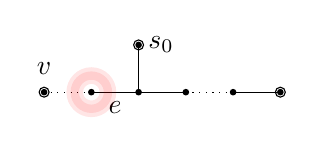
\begin{tikzpicture}[scale=0.6]
	\coordinate (1) at (0,0);
	\coordinate (A) at (1,0);
	\coordinate (B) at (2,0);
	\coordinate (C) at (3,0);
	\coordinate (D) at (4,0);
	\coordinate (2) at (5,0);
	\coordinate (3) at (2,1);
	
	\foreach \c in {1,2,3,A,B,C,D} {
		\fill (\c) circle (2pt);
	}
	\foreach \c in {1,2,3} {
		\draw (\c) circle (3pt);
	}

	\draw[dotted] (1) -- (A);
	\draw (A) -- node[below] {$e$} (B);
	\draw (B) -- (C);
	\draw[dotted] (C) -- (D);
	\draw (D) -- (2);
	\draw (B) -- (3);

	\node[above=0.1] at (1) {$v$};
	\node[right] at (3) {$s_0$};

	\draw[color=red, line width=6pt, opacity=0.1] (A) circle (10pt);
	\draw[color=red, line width=3pt, opacity=0.1] (A) circle (10pt);
\end{tikzpicture}
%\qquad\qquad
\end{minipage}
\begin{minipage}{0.45\textwidth}
\centering
% LABEL 2356
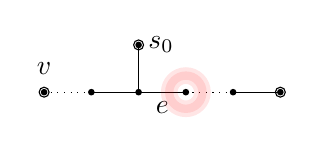
\begin{tikzpicture}[scale=0.6]
	\coordinate (1) at (0,0);
	\coordinate (A) at (1,0);
	\coordinate (B) at (2,0);
	\coordinate (C) at (3,0);
	\coordinate (D) at (4,0);
	\coordinate (2) at (5,0);
	\coordinate (3) at (2,1);
	
	\foreach \c in {1,2,3,A,B,C,D} {
		\fill (\c) circle (2pt);
	}
	\foreach \c in {1,2,3} {
		\draw (\c) circle (3pt);
	}

	\draw[dotted] (1) -- (A);
	\draw (A) -- (B);
	\draw (B) -- node[below] {$e$} (C);
	\draw[dotted] (C) -- (D);
	\draw (D) -- (2);
	\draw (B) -- (3);

	\node[above=0.1] at (1) {$v$};
	\node[right] at (3) {$s_0$};

	\draw[color=red, line width=6pt, opacity=0.1] (C) circle (10pt);
	\draw[color=red, line width=3pt, opacity=0.1] (C) circle (10pt);
\end{tikzpicture}
\end{minipage}
\caption{Edge $e \in T(s_0)$ with $\delta(e; v, s_0 ) = 1$ (left) and $\delta(e; v, s_0) = 0$ (right). The floating component of $T \setminus e$ is highlighted.}
\label{fig:e-delete-from-forest}
\end{figure}

Thus when multiplying the term \eqref{eq:delta-diff} by $(2 - \deg(u))$ and summing over all vertices $u$, we obtain
\[
	\sum_{u \in V} (2 - \deg(u)) \Big(\delta(e; v, \pi_T(u)) - \delta(e; v, u)\Big) 
	= \begin{cases}
	0 &\text{if } e \not \in T, \\
	2 - \degout(T \setminus e, *) &\text{if } e \in T(s_0) \text{ and } \delta(e; v, s_0) = 1, \\
	-(2 - \degout(T \setminus e, *)) &\text{if } e \in T(s_0) \text{ and } \delta(e; v, s_0) = 0 .
	\end{cases}
\]
Thus
\begin{multline}\label{eq:1}
	(D[S] \boldm)(v) - \sum_{T \in \trees} w(\overline{T}) \sum_{e \in E} \alpha_e \\
	= \sum_{T\in \trees} w(\overline{T}) \sum_{s_0 \in S} \left( \sum_{\substack{e \in T(s_0) \\ \delta(e;v,s_0) = 1}} \alpha_e ( 2 - \deg^o(T\setminus e,*)) 
	- \sum_{\substack{e  \in T(s_0) \\ \delta(e;v,s_0) = 0}} \alpha_e (2 - \deg^o(T\setminus e,*) ) \right)\\
	= \sum_{T\in \trees} w(\overline{T}) \sum_{e \in T} \alpha_e ( 2 - \deg^o(T\setminus e,*)) \left( \sum_{\substack{e \in T(s_0) \\ \delta(e;v,s_0) = 1}} 1
	- \sum_{\substack{e  \in T(s_0) \\ \delta(e;v,s_0) = 0}} 1 \right).
\end{multline}

We now rewrite the above expression in terms of $\forests_2(G;S)$,
observing that the deletion $T \setminus e$ is an $(S,*)$-rooted spanning forest of $G$, 
% since $e \in T$, 
and that the corresponding weights satisfy
\[
	w(\overline{F}) = \alpha_e \cdot w(\overline{T}) \qquad\text{if}\qquad F = T \setminus e.
\]
Thus
\begin{align*}
	\eqref{eq:1} &= \sum_{F \in \forests_2} w(\overline{F}) (2 - \deg^o(F,*)) \sum_{T\in \trees} \sum_{s_0 \in S} \left( \sum_{\substack{e \in T(s_0) \\ \delta(e; v,s_0) = 1}} \one(F = T \setminus e) -  \sum_{\substack{e \in T(s_0) \\ \delta(e; v,s_0) = 0}} \one(F = T \setminus e) \right) \\
	&= \sum_{F \in \forests_2} w(\overline{F}) (2 - \deg^o(F,*)) \Bigg( \#\{T \in \trees : F = T \setminus e \text{ for some } e \in T(s_0),\, \delta(e;v,s_0) = 1 \} \\
	&\qquad\qquad\qquad\qquad\qquad\qquad\qquad\quad - \#\{T \in \trees : F = T \setminus e \text{ for some } e \in T(s_0),\, \delta(e; v,s_0) = 0 \} \Bigg)
\end{align*}
Next, we note that $F = T \setminus e$ is equivalent to $T = F \cup e$, and in particular this only occurs when we choose the edge $e$ to be in the floating boundary $\partial F(*)$:

\begin{figure}[h]
% LABEL 2356
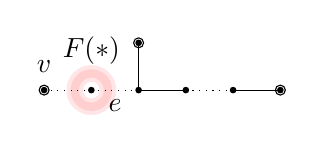
\begin{tikzpicture}[scale=0.6]
	\coordinate (1) at (0,0);
	\coordinate (A) at (1,0);
	\coordinate (B) at (2,0);
	\coordinate (C) at (3,0);
	\coordinate (D) at (4,0);
	\coordinate (2) at (5,0);
	\coordinate (3) at (2,1);
	
	\foreach \c in {1,2,3,A,B,C,D} {
		\fill (\c) circle (2pt);
	}
	\foreach \c in {1,2,3} {
		\draw (\c) circle (3pt);
	}

	\draw[dotted] (1) -- (A);
	\draw[dotted] (A) -- node[below] {$e$} (B);
	\draw (B) -- (C);
	\draw[dotted] (C) -- (D);
	\draw (D) -- (2);
	\draw (B) -- (3);

	\node[above=0.1] at (1) {$v$};
	\node[above=0.2] at (A) {$F(*)$};

	\draw[color=red, line width=6pt, opacity=0.1] (A) circle (10pt);
	\draw[color=red, line width=3pt, opacity=0.1] (A) circle (10pt);
\end{tikzpicture}
\qquad\qquad
% LABEL 2356
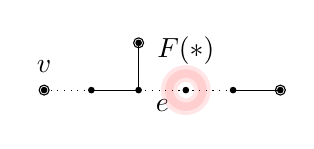
\begin{tikzpicture}[scale=0.6]
	\coordinate (1) at (0,0);
	\coordinate (A) at (1,0);
	\coordinate (B) at (2,0);
	\coordinate (C) at (3,0);
	\coordinate (D) at (4,0);
	\coordinate (2) at (5,0);
	\coordinate (3) at (2,1);
	
	\foreach \c in {1,2,3,A,B,C,D} {
		\fill (\c) circle (2pt);
	}
	\foreach \c in {1,2,3} {
		\draw (\c) circle (3pt);
	}

	\draw[dotted] (1) -- (A);
	\draw (A) -- (B);
	\draw[dotted] (B) -- node[below] {$e$} (C);
	\draw[dotted] (C) -- (D);
	\draw (D) -- (2);
	\draw (B) -- (3);

	\node[above=0.1] at (1) {$v$};
	\node[above=0.2] at (C) {$F(*)$};
	
	\draw[color=red, line width=6pt, opacity=0.1] (C) circle (10pt);
	\draw[color=red, line width=3pt, opacity=0.1] (C) circle (10pt);
\end{tikzpicture}
\caption{Edge $e \in \partial F(*)$ with $\delta(e; v, F(*)) = 0$ (left) and $\delta(e; v, F(*)) = 1$ (right). The floating component $F(*)$ is highlighted.}
\end{figure}

%\begin{multline}
%	\eqref{eq:1} = \sum_{F \in \forests_2} w(\overline{F}) (2 - \deg^o(F,*))  \sum_{e \in \partial F(*)} \Bigg( \sum_{\substack{s_0 \in S \\ \delta(e; v, s_0) = 0}} \; \sum_{\substack{T \in \trees \\ e \in T(s_0)}} \one(T = F \cup e) \\
%	- \sum_{\substack{s_0 \in S \\ \delta(e; v, s_0) = 1}} \; \sum_{\substack{T \in \trees \\ e \in T(s_0)}} \one(T = F \cup e) \Bigg).
%\end{multline}
Now for any $e \not\in F$, let $\delta(e; v, F(*)) = \delta(e; v, x)$ for any $x \in F(*)$, i.e.
\[
	\delta(e; v, F(*)) = \begin{cases}
	1 &\text{if $e$ lies on path from $v$ to $F(*)$}, \\
	0 &\text{otherwise}.
	\end{cases}
\]
The condition $F = T \setminus e$ for some $e \in T(s_0)$ with $\delta(e; v, s_0) = 1$ (resp. $\delta(e; v, s_0) = 0$) is equivalent to $T = F \cup e$ for some $e \in \partial F(*)$ with $\delta(e; v, F(*)) = 0$ (resp. $\delta(e; v, F(*)) = 1$).
Thus
\begin{multline}
	\eqref{eq:1} = \sum_{F \in \forests_2} w(\overline{F}) (2 - \deg^o(F,*))  \Bigg( \#\{e \in \partial F(*) : \delta(e; v, F(*)) = 0 \}  \\
	- \#\{e \in \partial F(*) : \delta(e; v, F(*)) = 1 \}  \Bigg).
\end{multline}
Finally, we observe that for any forest $F$ in $\forests_2(G;S)$,
there is exactly one edge $e$ in the boundary $\partial F(*)$ of the floating component which satisfies $\delta(e; v, F(*)) = 1$, namely the unique boundary edge on the path from the floating component $F(*)$ to $v$.
Hence
\[
	\#\{e \in \partial F(*) : \delta(e;v, F(*)) = 1 \} = 1
\qquad\text{and}\qquad
	\#\{e \in \partial (F,*) : \delta(e;v, F(*)) = 0 \} = \deg^o(F,*) - 1 .
\]
Thus the previous expression \eqref{eq:1} simplifies as
\begin{align*}
	\eqref{eq:1} &= \sum_{F \in \forests_2} w(\overline{F}) (2 - \degout(F,*))  \Big( (\degout(F,*) - 1)  - (1) \Big) \\
	% &\qquad - \sum_{F \in \forests_2} w(\overline{F}) (2 - \degout(F,*)) (1) \\
	&= - \!\sum_{F \in \forests_2} w(\overline{F}) (2 - \degout(F,*))^2 .
\end{align*}
as desired.
\end{proof}

\begin{figure}[h]
% LABEL 1345
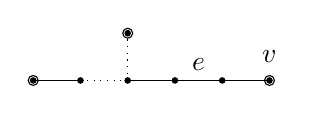
\begin{tikzpicture}[scale=0.6]
	\coordinate (1) at (0,0);
	\coordinate (A) at (1,0);
	\coordinate (B) at (2,0);
	\coordinate (C) at (3,0);
	\coordinate (D) at (4,0);
	\coordinate (2) at (5,0);
	\coordinate (3) at (2,1);
	
	\foreach \c in {1,2,3,A,B,C,D} {
		\fill (\c) circle (2pt);
	}
	\foreach \c in {1,2,3} {
		\draw (\c) circle (3pt);
	}

	\draw (1) -- (A);
	\draw[dotted] (A) -- (B);
	\draw (B) -- (C);
	\draw (C) -- node[above] {$e$} (D);
	\draw (D) -- (2);
	\draw[dotted] (B) -- (3);

	\node[above=0.1] at (2) {$v$};
\end{tikzpicture}
\qquad
% LABEL 1346
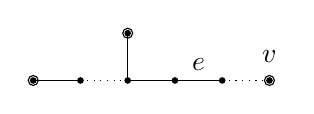
\begin{tikzpicture}[scale=0.6]
	\coordinate (1) at (0,0);
	\coordinate (A) at (1,0);
	\coordinate (B) at (2,0);
	\coordinate (C) at (3,0);
	\coordinate (D) at (4,0);
	\coordinate (2) at (5,0);
	\coordinate (3) at (2,1);
	
	\foreach \c in {1,2,3,A,B,C,D} {
		\fill (\c) circle (2pt);
	}
	\foreach \c in {1,2,3} {
		\draw (\c) circle (3pt);
	}

	\draw (1) -- (A);
	\draw[dotted] (A) -- (B);
	\draw (B) -- (C);
	\draw (C) -- node[above] {$e$} (D);
	\draw[dotted] (D) -- (2);
	\draw (B) -- (3);

	\node[above=0.1] at (2) {$v$};
\end{tikzpicture}
\qquad
% LABEL 1356
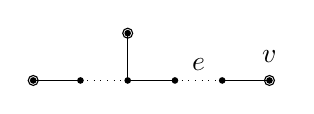
\begin{tikzpicture}[scale=0.6]
	\coordinate (1) at (0,0);
	\coordinate (A) at (1,0);
	\coordinate (B) at (2,0);
	\coordinate (C) at (3,0);
	\coordinate (D) at (4,0);
	\coordinate (2) at (5,0);
	\coordinate (3) at (2,1);
	
	\foreach \c in {1,2,3,A,B,C,D} {
		\fill (\c) circle (2pt);
	}
	\foreach \c in {1,2,3} {
		\draw (\c) circle (3pt);
	}

	\draw (1) -- (A);
	\draw[dotted] (A) -- (B);
	\draw (B) -- (C);
	\draw[dotted] (C) -- node[above] {$e$} (D);
	\draw (D) -- (2);
	\draw (B) -- (3);

	\node[above=0.1] at (2) {$v$};
\end{tikzpicture}
\caption{Components rooted in $S(G\setminus e)^{\overline v}$.}
\end{figure}
 
%\note{MOVE TO REMARK? If $e \in \conv(G,S)$, then $S(G\backslash e)^{\overline v}$ is nonempty and }
%
%\begin{rmk} \,\note{consider deleting}
%The set $\forests_2(G;S)$ of $(S,*)$-rooted spanning forests of $G$ can be partitioned into two types: ``active'' and ``inactive''.
%\[
%	\forests_2(G;S) = \forests_2^{in}(G;S) \sqcup \forests_2^{out}(G;S),
%\]
%where
%\[
%	\forests_2^{in}(G;S)  = \{ F \in \forests_2(G;S) \text{ such that } \deg^o(*,F) \geq 2\},
%\]
%$$
%\forests_2^{out}(G;S)  = \{ F \in \forests_2(G;S) \text{ such that } \deg^o(*,F) = 1\}.
%$$
%\end{rmk}

Finally we can prove our main theorem: for any nonempty subset $S \subset V(G)$,
\begin{equation}
\label{eq:w-main-later}
	\det D[S] = (-1)^{|S|-1} 2^{|S|-2} \left( \sum_{E(G)}\alpha_e \sum_{\trees(G;S)} w(\overline{T}) - \sum_{\forests_2(G;S)} (\degout(F,*) - 2)^2 w(\overline{F}) \right).
\end{equation}
\begin{proof}[Proof of Theorem~\ref{thm:w-main}]
First, suppose $|S| = 1$.
Then $D[S]$ is the zero matrix, and we must show that the right-hand side is zero.
Since $G$ is a tree, $\trees(G; \{v\})$ consists of the tree $G$ itself, with co-weight $w(\overline{G}) = 1$.
Moreover, the subgraphs in $\forests_2(G; \{v\})$ are precisely the tree splits $G \setminus e$, and for each $F = G \setminus e$ we have 
$w(\overline{F}) = \alpha_e$ and
$\degout(F, *) - 2 = -1$.
This shows that the right-hand size of \eqref{eq:w-main-later} is zero.

Next, suppose $|S| \geq 2$.
Proposition~\ref{prop:distance-sub-nonsingular} states that $D[S]$ is nonsingular, so we may use the inverse matrix identity
\begin{equation}\label{eq:cof-invsere-sum}
	\bone^\tr D[S]^{-1} \bone =
	\frac{\cof D[S]}{\det D[S]}. 
\end{equation}
Let $\boldm = \boldm(G; S)$ denote the vector \eqref{eq:m-vector}.
By 
Proposition~\ref{prop:m-sum} (a) and
% Bapat--Sivasubramanian~\cite[Theorem X]{bapat-sivasubramanian},
Theorem~\ref{thm:distance-sub-cof},
\[
	\bone^\tr \boldm 
	= 2 \sum_{T \in \trees(G;S)} w(\overline{T})
	= \frac{\cof D[S]}{(-1)^{1 - |S|} 2^{2 - |S|} }.
\]
Theorem~\ref{thm:m-distance-product} states that $D[S] \boldm = \lambda \bone$
for some constant $\lambda$,
which is nonzero since $D[S]$ is invertible and $\boldm$ is nonzero, c.f. Proposition~\ref{prop:m-sum} (b).
Hence
\begin{equation}\label{eq:inverse-sum-entries}
	% \frac{\cof D[S]}{\det D[S]} = 
	\bone^\tr D[S]^{-1} \bone
	= \lambda^{-1} \bone^\tr \boldm
	= \frac{\cof D[S]}{(-1)^{|S| - 1} 2^{|S| - 1} \lambda} .
\end{equation}
Comparing \eqref{eq:cof-invsere-sum} with \eqref{eq:inverse-sum-entries} gives the desired result,
$\det D[S] = (-1)^{|S| - 1} 2^{|S| - 1} \lambda$.
\end{proof}

\begin{proof}[Proof of Theorem~\ref{thm:main}]
Set all weights $\alpha_e$ to $1$ in Theorem~\ref{thm:w-main}.
In this case, the weights $w(\overline{T}) = 1$ and $w(\overline{F}) = 2$ for all forests $T$ and $F$,
and 
\[
n - 1 = |E(G)|, 
\qquad \kappa_1(G; S) = | \trees(G;S)|.
%\qquad \kappa_2(G; S) = | \forests_2(G; S)| .
\]
\end{proof}

\begin{rmk}
It is worth observing that depending on the chosen subset $S \subset V$, the distances appearing in the submatrix $D[S]$ may ignore a large part of the ambient tree $G$.
We could instead replace $G$ by the subtree  $\conv(S,G)$ consisting of the union of all paths between vertices in $S$,
which we call the {\em convex hull} of $S \subset G$.
To apply formula \eqref{eq:main} or \eqref{eq:w-main} ``efficiently,''
we should replace $G$ on the right-hand side with the subtree $\conv(S,G)$.
However, the formulas as stated are true even without this replacement due to cancellation of terms.
\end{rmk}

\section{Physical interpretation}

If we consider $G$ as a network of wires with edge $e$ containing a resistor of resistance $\alpha_e$,
which is grounded at all nodes in $S$,
then $\boldm_S$ has an interpretation as current flow: 
it records the currents flowing to $S$
when current enters the vertices in the amount $2 - \deg v$
for each $v\not\in S$.

\subsection{Alternate proof}

Let $\mathbf{1}$ denote the all-ones vector.
When we choose a subset $S \subset V(G)$, we no longer have a single ``obvious'' replacement for $\boldm$ inside $\RR^S$.
Instead, we can take an average over $S$-rooted spanning forests.

In the outline above, our first goal is to find a ``special'' vector $ \boldm\in \RR^S$ satisfying $D[S] \boldm = \lambda \mathbf{1}$.
We can approach this first goal as follows: 
consider $\RR^S$ inside the larger vector space $\RR^V = \RR^S \oplus \RR^{V\setminus S}$,
and let $\pi_S$ denote the projection from $\RR^V$ to $\RR^S$.
We wish to find vectors $\mathbf{n}_i \in \RR^{V}$ satisfying
$\pi_S( D \mathbf{n}_i) = \lambda_i \mathbf{1}$.
OR, $D \mathbf{n}_i = \lambda_i \mathbf{1}^S \oplus (-)$.
By finding sufficiently many such vectors $\mathbf{n}_i$,
we can hope to find a linear combination that lies inside $\RR^S \oplus \{0\}$.
% $D \mathbf{n} = (\lambda \mathbf{1}_S) \oplus (-)$.

\begin{prop}
\label{prop:n-vector}
Suppose $v \in V \setminus S$.
For each $s_j \in S$, let $\mu(v,s_j) = $ current flowing to $s_j$
when 
$G$ is grounded at $S$
and 
one unit of current enters $G$ at $v$.
Explicitly,
\begin{equation*}
\mu(v,s) =  \frac{\text{\# of $S$-rooted spanning forests of $G$ whose $s_j$-component contains $v$}}{\text{\# of $S$-rooted spanning forests of $G$}}
% = (\kappa(..))/(\kappa(G/S))
\end{equation*}
\[
= \frac{\sum_{\trees(G/S)} \mathds{1}(v \in T(s))}{\kappa(G/S)}
\]
\[
= \frac{\kappa_{r}(s_1|\cdots|s_j v| \cdots|s_r)}{\kappa_r(s_1|\cdots|s_r)}
\]
Consider the vector $\mathbf{n} = \mathbf{n}(G;S,v) \in \RR^V$ defined by
\[
	\mathbf{n}_v = 1,\qquad
	\mathbf{n}_s = -\mu(v,s) \text{ if }s \in S, \qquad
	\mathbf{n}_w = 0 \text{ if } w \not\in S \cup v
\]
Then $D\mathbf{n}$ is constant on $S$, i.e. $\pi_S( D \mathbf{n}) = \lambda \mathbf{1}$ for some $\lambda$.
\end{prop}
\begin{proof}[Proof sketch]
For any $s, s' \in S$, consider tracking the value of $D \mathbf{n}$ along path from $s$ to $s'$. 
The value of $D \mathbf{n}$ changes according to current flow in the corresponding network, i.e. $D \mathbf{n}$ records electrical potential.
By assumption $S$ is grounded, so $D\mathbf{n}$ takes the same value at $s$ and $s'$.
\end{proof}

\begin{thm}
Let $G$ be a tree, $S$ a nonempty subset of vertices,
and $D[S]$ the corresponding submatrix of the distance matrix of $G$.
Suppose $\boldm = \boldm(G;S) \in \RR^{S}$ is defined by \eqref{eq:m-vector};
\begin{equation}
\boldm(G;S)_v = \sum_{T \in \trees(G;S)} w(\overline{T}) \sum_{u \in T(v)} (2 - \deg u) 
= \sum_{T \in \trees(G;S)} w(\overline{T}) (2 - \degout(T,v)) .
\end{equation}
Then $D[S] \boldm = \lambda \bone$
for some constant $\lambda$.
\end{thm}
\begin{proof}
The vector $\boldm = \boldm(G;S)$ can be expressed as a linear combination
\begin{align}
	\boldm (G;S)
	&= \kappa(G;S) \left( \sum_{v \in V}(2 - \deg v) {\bolddelta}(v) 
	- \sum_{v \in V \setminus S} (2 - \deg v) \mathbf{n}(G;S,v) 
	\right) \\
	&= \kappa(G;S) \left( \boldm(G;V) - \sum_{v\in V\setminus S} (2 - \deg v) \boldn(G;S,v) \right)
\end{align}
\note{TODO: elaborate on this equation}
From Proposition~\ref{prop:m-distance-warmup} we know that $D \boldm(G;V)$ is constant on $V$,
and from Proposition~\ref{prop:n-vector} we know that $D \boldn(G;S,v)$ is constant on $S$.
Hence by linearity, $D \boldm(G;S)$ is constant on $S$.
\end{proof}

\begin{prop}
Let $G = (V,E)$ be a tree, and $S \subset V$.
Suppose we label $S = \{s_1, \ldots, s_r\}$
and $V \setminus S = \{t_1, \ldots, t_{n-r}\}$.
For each $t_i \in V\setminus S$,
consider
$\mathbf{f}_i  \in \RR^V$
defined by
\end{prop}

\begin{eg}
If 
$$
D[S \cup t] = \begin{bmatrix}
0 & a & b & c \\
a & 0 & a + b & a + c \\
b & a + b & 0 & b + c \\
c & a + c & b + c & 0
\end{bmatrix}
$$
then
$$
 \begin{bmatrix}
0 & a & b & c \\
a & 0 & a + b & a + c \\
b & a + b & 0 & b + c \\
c & a + c & b + c & 0
\end{bmatrix}
\begin{bmatrix}
ab + ac + bc \\ -bc \\ -ac \\ -ab 
\end{bmatrix}
= \begin{bmatrix}
-3abc \\ -abc \\ -abc \\ -abc
\end{bmatrix}
$$
\end{eg}

\subsection{Symanzik polynomials}

We note that the expression in the main theorem, Theorem~\ref{thm:w-main}, is related to Symanzik polynomials, which we recall here.

Given a graph $G = (V, E)$, the {\em first Symanzik polynomial} is the homogeneous polynomial in edge-indexed variables $\underline{x} = \{x_e : e \in E\}$ defined by
\[
	\psi_G(\underline{x}) = \sum_{T \in \trees(G)} \prod_{e \not \in T} x_e ,
\]
where $\trees(G)$ denotes the set of spanning trees of $G$.

Consider a ``momentum'' function $p: V \to \RR$ which satisfies $\sum_{v \in V} p(v) = 0$.
Then the second Symanzik polynomial is
\[
	\varphi_G(p; \underline{x}) = \sum_{F \in \forests_2(G)} \left(\sum_{v \in F_1} p(v) \right)^2 \prod_{e \not\in F} x_e ,
\]
where $\forests_2(G)$ is the set of two-component spanning forests of $G$, and $F_1$ denotes one of the components of $F$.
It doesn't matter which component we label as $F_1$, due to the momemtum constraint $\sum_{v \in V} p(v) = 0$.
% If $F_2$ denotes the other component of $F$, the constraint $\sum_{v \in V} p(v) = 0$ implies that
% $\left(\sum_{v \in F_1} p(v) \right)^2 = \left(\sum_{v \in F_2} p(v) \right)^2$.

Theorem statement:
\[
	\det D[S] = (-1)^{|S|-1} 2^{|S|-2} \left( \sum_{E(G)}\alpha_e \sum_{\trees(G;S)} w(\overline{T}) - \sum_{\forests_2(G;S)} (\degout(F,*) - 2)^2 w(\overline{F}) \right).
\]
\[
	\frac{\det D[S]}{\cof D[S]} = \frac12 \left( \sum_{e \in E} \alpha_e - \frac{\sum_{F \in \forests_2(G; S)} w(\overline{F}) (\degout(F,*) - 2)^2}{\sum_{T \in \trees(G; S)} w(\overline{T})} \right)
\]
In terms of Symanzik polynomials, let $\psi$ and $\varphi$ denote the first and second Symanzik polynomials of the quotient graph $G/S$.
We have
\[
	\det D[S] = (-1)^{|S|-1} 2^{|S|-2} \left( \sum_{E(G)}\alpha_e \, \psi_{(G/S)}(\underline{\alpha}) - \phi_{(G/S)}(p; \underline{\alpha}) \right).
\]
and
\[
	\frac{\det D[S]}{\cof D[S]} = \frac12 \left( \sum_{e \in E} \alpha_e - \frac{\varphi_{(G/S)}(p; \underline{\alpha})}{\psi_{(G/S)}(\underline{\alpha})} \right)
\]
with momentum function $p(v) = \deg(v) - 2$ for $v \not \in S$.


\section{Examples}

\begin{eg}
Suppose $G$ is a tree consisting of three paths joined at a central vertex.
Let $S$ consist of the central vertex, and the three endpoints of the paths. 
The corresponding minor of the distance matrix is
\[
	D[S] = \begin{bmatrix}
	0 & a & b & c \\
	a & 0 & a + b & a + c \\
	b & a + b & 0 & b + c \\
	c & a + c & b + c & 0
	\end{bmatrix}
	\sim \begin{bmatrix}
	0 & a & b & c \\
	a & -a & a  & a \\
	b & b & -b & b \\
	c & c & c & -c
	\end{bmatrix}
	\sim \begin{bmatrix}
	0 & a & b & c \\
	a & -2a & 0 & 0 \\
	b & 0 & -2b & 0 \\
	c & 0 & 0 & -2c
	\end{bmatrix}.
\]
The determinant is
\begin{align*}
	\det D[S] = -4(a+b+c)abc.
\end{align*}
\end{eg}

\begin{eg}
Suppose $\Gamma$ is a tripod with lengths $a,b,c$ and corresponding leaf vertices $u,v,w$.
\[
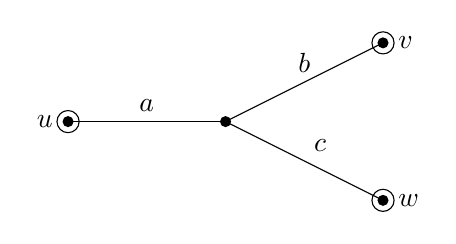
\begin{tikzpicture}
	\coordinate (u) at (-2,0);
	\coordinate (v) at (2,1);
	\coordinate (w) at (2,-1);
	\coordinate (o) at (0,0);

	\draw (o) -- (u);
	\draw (v) -- (o) -- (w);

	\foreach \c in {u, v, w, o} {
		\fill (\c) circle (2pt);
	}
	\foreach \c in {u, v, w} {
		\draw (\c) circle (4pt);
	}
	
	\node[left=2pt] at (u) {$u$};
	\node[right=2pt] at (v) {$v$};
	\node[right=2pt] at (w) {$w$};

	\node[above] at (-1,0) {$a$};
	\node[above] at (1,0.5) {$b$};
	\node[above right] at (1,-0.5) {$c$};
\end{tikzpicture}
\]
Let $S = \{u,v,w\}$.
Then 
\[
	D[S] = \begin{bmatrix}
	0 & a + b & a + c \\
	a + b & 0 & b + c \\
	a + c & b + c & 0
	\end{bmatrix}.
\]
and
\begin{align*}
	\det D[S] &= 2(a+b)(a+c)(b+c) 
	= 2\left( (a+b+c)(ab + ac + bc) - abc \right).
\end{align*}
The ``special vector'' that satisfies $D[S] \boldm = \lambda \mathbf{1}$ in this example is 
$$
\boldm = \begin{bmatrix} a(b + c) & b(a + c) & c(a + b) \end{bmatrix}^\tr .
$$
\end{eg}

\begin{eg}
Suppose $G$ is the tree with unit edge lengths shown below, with five leaf vertices.
\[
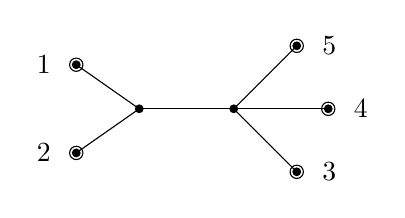
\begin{tikzpicture}[scale=0.8]
	\coordinate (1) at (-2,0.7);
	\coordinate (2) at (-2,-0.7);
	\coordinate (3) at (1.5,-1);
	\coordinate (4) at (2,0);
	\coordinate (5) at (1.5,1);
	\coordinate (A) at (-1,0);
	\coordinate (B) at (0.5,0);
	
	\foreach \c in {1,2,3,4,5,A,B} {
		\fill (\c) circle (2pt);
	}
	\foreach \c in {1,2,3,4,5} {
		\draw (\c) circle (3pt);
	}

	\draw (A) -- (1);
	\draw (A) -- (2);
	\draw (B) -- (3);
	\draw (B) -- (4);
	\draw (B) -- (5);
	\draw (A) -- (B);
	
	\foreach \c/\d in {1/left,2/left,3/right,4/right,5/right} {
		\node[\d=0.2] at (\c) {$\c$};
	}
\end{tikzpicture}
\]
Let $S$ denote the set of five leaf vertices. Then
$$
D[S] = \begin{bmatrix}
0 & 2 & 3 & 3 & 3 \\
2 & 0 & 3 & 3 & 3 \\
3 & 3 & 0 & 2 & 2 \\
3 & 3 & 2 & 0 & 2 \\
3 & 3 & 2 & 2 & 0
\end{bmatrix}.
$$
There are $11$ forests in $\trees(G;S)$:
\[
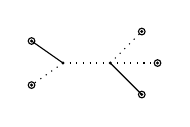
\begin{tikzpicture}[scale=0.4]
	\coordinate (1) at (-2,0.7);
	\coordinate (2) at (-2,-0.7);
	\coordinate (3) at (1.5,-1);
	\coordinate (4) at (2,0);
	\coordinate (5) at (1.5,1);
	\coordinate (A) at (-1,0);
	\coordinate (B) at (0.5,0);
	
	\foreach \c in {1,2,3,4,5,A,B} {
		\fill (\c) circle (1.5pt);
	}
	\foreach \c in {1,2,3,4,5} {
		\draw (\c) circle (3pt);
	}

	\draw (A) -- (1);
	\draw[dotted] (A) -- (2);
	\draw (B) -- (3);
	\draw[dotted] (B) -- (4);
	\draw[dotted] (B) -- (5);
	\draw[dotted] (A) -- (B);
\end{tikzpicture}
\qquad
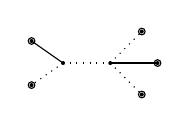
\begin{tikzpicture}[scale=0.4]
	\coordinate (1) at (-2,0.7);
	\coordinate (2) at (-2,-0.7);
	\coordinate (3) at (1.5,-1);
	\coordinate (4) at (2,0);
	\coordinate (5) at (1.5,1);
	\coordinate (A) at (-1,0);
	\coordinate (B) at (0.5,0);
	
	\foreach \c in {1,2,3,4,5,A,B} {
		\fill (\c) circle (1.8pt);
	}
	\foreach \c in {1,2,3,4,5} {
		\draw (\c) circle (3pt);
	}

	\draw (A) -- (1);
	\draw[dotted] (A) -- (2);
	\draw[dotted] (B) -- (3);
	\draw (B) -- (4);
	\draw[dotted] (B) -- (5);
	\draw[dotted] (A) -- (B);
\end{tikzpicture}
\qquad
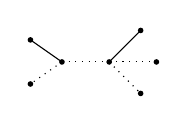
\begin{tikzpicture}[scale=0.4]
	\filldraw[black] (-2,0.7) coordinate (1) circle (2pt);
	\filldraw[black] (-2,-0.7) coordinate (2) circle (2pt);
	\filldraw[black] (1.5,-1) coordinate (3) circle (2pt);
	\filldraw[black] (2,0) coordinate (4) circle (2pt);
	\filldraw[black] (1.5,1) coordinate (5) circle (2pt);
	\filldraw[black] (-1,0) coordinate (A) circle (2pt);
	\filldraw[black] (0.5,0) coordinate (B) circle (2pt);

	\draw (A) -- (1);
	\draw[dotted] (A) -- (2);
	\draw[dotted] (B) -- (3);
	\draw[dotted] (B) -- (4);
	\draw (B) -- (5);
	\draw[dotted] (A) -- (B);
\end{tikzpicture}
\qquad
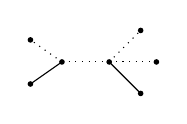
\begin{tikzpicture}[scale=0.4]
	\filldraw[black] (-2,0.7) coordinate (1) circle (2pt);
	\filldraw[black] (-2,-0.7) coordinate (2) circle (2pt);
	\filldraw[black] (1.5,-1) coordinate (3) circle (2pt);
	\filldraw[black] (2,0) coordinate (4) circle (2pt);
	\filldraw[black] (1.5,1) coordinate (5) circle (2pt);
	\filldraw[black] (-1,0) coordinate (A) circle (2pt);
	\filldraw[black] (0.5,0) coordinate (B) circle (2pt);

	\draw[dotted] (A) -- (1);
	\draw (A) -- (2);
	\draw (B) -- (3);
	\draw[dotted] (B) -- (4);
	\draw[dotted] (B) -- (5);
	\draw[dotted] (A) -- (B);
\end{tikzpicture}
\qquad
\begin{tikzpicture}[scale=0.4]
	\filldraw[black] (-2,0.7) coordinate (1) circle (2pt);
	\filldraw[black] (-2,-0.7) coordinate (2) circle (2pt);
	\filldraw[black] (1.5,-1) coordinate (3) circle (2pt);
	\filldraw[black] (2,0) coordinate (4) circle (2pt);
	\filldraw[black] (1.5,1) coordinate (5) circle (2pt);
	\filldraw[black] (-1,0) coordinate (A) circle (2pt);
	\filldraw[black] (0.5,0) coordinate (B) circle (2pt);

	\draw[dotted] (A) -- (1);
	\draw (A) -- (2);
	\draw[dotted] (B) -- (3);
	\draw (B) -- (4);
	\draw[dotted] (B) -- (5);
	\draw[dotted] (A) -- (B);
\end{tikzpicture}
\qquad
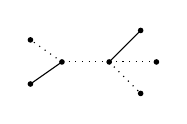
\begin{tikzpicture}[scale=0.4]
	\filldraw[black] (-2,0.7) coordinate (1) circle (2pt);
	\filldraw[black] (-2,-0.7) coordinate (2) circle (2pt);
	\filldraw[black] (1.5,-1) coordinate (3) circle (2pt);
	\filldraw[black] (2,0) coordinate (4) circle (2pt);
	\filldraw[black] (1.5,1) coordinate (5) circle (2pt);
	\filldraw[black] (-1,0) coordinate (A) circle (2pt);
	\filldraw[black] (0.5,0) coordinate (B) circle (2pt);

	\draw[dotted] (A) -- (1);
	\draw (A) -- (2);
	\draw[dotted] (B) -- (3);
	\draw[dotted] (B) -- (4);
	\draw (B) -- (5);
	\draw[dotted] (A) -- (B);
\end{tikzpicture}
\]
\[
\begin{tikzpicture}[scale=0.4]
	\filldraw[black] (-2,0.7) coordinate (1) circle (2pt);
	\filldraw[black] (-2,-0.7) coordinate (2) circle (2pt);
	\filldraw[black] (1.5,-1) coordinate (3) circle (2pt);
	\filldraw[black] (2,0) coordinate (4) circle (2pt);
	\filldraw[black] (1.5,1) coordinate (5) circle (2pt);
	\filldraw[black] (-1,0) coordinate (A) circle (2pt);
	\filldraw[black] (0.5,0) coordinate (B) circle (2pt);

	\draw (A) -- (1);
	\draw[dotted] (A) -- (2);
	\draw[dotted] (B) -- (3);
	\draw[dotted] (B) -- (4);
	\draw[dotted] (B) -- (5);
	\draw (A) -- (B);
\end{tikzpicture}
\qquad
\begin{tikzpicture}[scale=0.4]
	\filldraw[black] (-2,0.7) coordinate (1) circle (2pt);
	\filldraw[black] (-2,-0.7) coordinate (2) circle (2pt);
	\filldraw[black] (1.5,-1) coordinate (3) circle (2pt);
	\filldraw[black] (2,0) coordinate (4) circle (2pt);
	\filldraw[black] (1.5,1) coordinate (5) circle (2pt);
	\filldraw[black] (-1,0) coordinate (A) circle (2pt);
	\filldraw[black] (0.5,0) coordinate (B) circle (2pt);

	\draw[dotted] (A) -- (1);
	\draw (A) -- (2);
	\draw[dotted] (B) -- (3);
	\draw[dotted] (B) -- (4);
	\draw[dotted] (B) -- (5);
	\draw (A) -- (B);
\end{tikzpicture}
\qquad
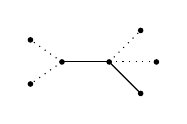
\begin{tikzpicture}[scale=0.4]
	\filldraw[black] (-2,0.7) coordinate (1) circle (2pt);
	\filldraw[black] (-2,-0.7) coordinate (2) circle (2pt);
	\filldraw[black] (1.5,-1) coordinate (3) circle (2pt);
	\filldraw[black] (2,0) coordinate (4) circle (2pt);
	\filldraw[black] (1.5,1) coordinate (5) circle (2pt);
	\filldraw[black] (-1,0) coordinate (A) circle (2pt);
	\filldraw[black] (0.5,0) coordinate (B) circle (2pt);

	\draw[dotted] (A) -- (1);
	\draw[dotted] (A) -- (2);
	\draw (B) -- (3);
	\draw[dotted] (B) -- (4);
	\draw[dotted] (B) -- (5);
	\draw (A) -- (B);
\end{tikzpicture}
\qquad
\begin{tikzpicture}[scale=0.4]
	\filldraw[black] (-2,0.7) coordinate (1) circle (2pt);
	\filldraw[black] (-2,-0.7) coordinate (2) circle (2pt);
	\filldraw[black] (1.5,-1) coordinate (3) circle (2pt);
	\filldraw[black] (2,0) coordinate (4) circle (2pt);
	\filldraw[black] (1.5,1) coordinate (5) circle (2pt);
	\filldraw[black] (-1,0) coordinate (A) circle (2pt);
	\filldraw[black] (0.5,0) coordinate (B) circle (2pt);

	\draw[dotted] (A) -- (1);
	\draw[dotted] (A) -- (2);
	\draw[dotted] (B) -- (3);
	\draw (B) -- (4);
	\draw[dotted] (B) -- (5);
	\draw (A) -- (B);
\end{tikzpicture}
\qquad
\begin{tikzpicture}[scale=0.4]
	\filldraw[black] (-2,0.7) coordinate (1) circle (2pt);
	\filldraw[black] (-2,-0.7) coordinate (2) circle (2pt);
	\filldraw[black] (1.5,-1) coordinate (3) circle (2pt);
	\filldraw[black] (2,0) coordinate (4) circle (2pt);
	\filldraw[black] (1.5,1) coordinate (5) circle (2pt);
	\filldraw[black] (-1,0) coordinate (A) circle (2pt);
	\filldraw[black] (0.5,0) coordinate (B) circle (2pt);

	\draw[dotted] (A) -- (1);
	\draw[dotted] (A) -- (2);
	\draw[dotted] (B) -- (3);
	\draw[dotted] (B) -- (4);
	\draw (B) -- (5);
	\draw (A) -- (B);
\end{tikzpicture}
\]
There are $6$ forests in $\forests_2(G;S)$:
\[
\begin{tikzpicture}[scale=0.4]
	\coordinate (1) at (-2,0.7);
	\coordinate (2) at (-2,-0.7);
	\coordinate (3) at (1.5,-1);
	\coordinate (4) at (2,0);
	\coordinate (5) at (1.5,1);
	\coordinate (A) at (-1,0);
	\coordinate (B) at (0.5,0);
	
	\foreach \c in {1,2,3,4,5,A,B} {
		\fill (\c) circle (1.5pt);
	}
	\foreach \c in {1,2,3,4,5} {
		\draw (\c) circle (3pt);
	}

	\draw[dotted] (A) -- (1);
	\draw[dotted] (A) -- (2);
	\draw (B) -- (3);
	\draw[dotted] (B) -- (4);
	\draw[dotted] (B) -- (5);
	\draw[dotted] (A) -- (B);
\end{tikzpicture}
\qquad
\begin{tikzpicture}[scale=0.4]
	\coordinate (1) at (-2,0.7);
	\coordinate (2) at (-2,-0.7);
	\coordinate (3) at (1.5,-1);
	\coordinate (4) at (2,0);
	\coordinate (5) at (1.5,1);
	\coordinate (A) at (-1,0);
	\coordinate (B) at (0.5,0);
	
	\foreach \c in {1,2,3,4,5,A,B} {
		\fill (\c) circle (1.5pt);
	}
	\foreach \c in {1,2,3,4,5} {
		\draw (\c) circle (3pt);
	}

	\draw[dotted] (A) -- (1);
	\draw[dotted] (A) -- (2);
	\draw[dotted] (B) -- (3);
	\draw (B) -- (4);
	\draw[dotted] (B) -- (5);
	\draw[dotted] (A) -- (B);
\end{tikzpicture}
\qquad
\begin{tikzpicture}[scale=0.4]
	\coordinate (1) at (-2,0.7);
	\coordinate (2) at (-2,-0.7);
	\coordinate (3) at (1.5,-1);
	\coordinate (4) at (2,0);
	\coordinate (5) at (1.5,1);
	\coordinate (A) at (-1,0);
	\coordinate (B) at (0.5,0);
	
	\foreach \c in {1,2,3,4,5,A,B} {
		\fill (\c) circle (1.5pt);
	}
	\foreach \c in {1,2,3,4,5} {
		\draw (\c) circle (3pt);
	}

	\draw[dotted] (A) -- (1);
	\draw[dotted] (A) -- (2);
	\draw[dotted] (B) -- (3);
	\draw[dotted] (B) -- (4);
	\draw (B) -- (5);
	\draw[dotted] (A) -- (B);
\end{tikzpicture}
\]
\[
\begin{tikzpicture}[scale=0.4]
	\coordinate (1) at (-2,0.7);
	\coordinate (2) at (-2,-0.7);
	\coordinate (3) at (1.5,-1);
	\coordinate (4) at (2,0);
	\coordinate (5) at (1.5,1);
	\coordinate (A) at (-1,0);
	\coordinate (B) at (0.5,0);
	
	\foreach \c in {1,2,3,4,5,A,B} {
		\fill (\c) circle (1.5pt);
	}
	\foreach \c in {1,2,3,4,5} {
		\draw (\c) circle (3pt);
	}

	\draw (A) -- (1);
	\draw[dotted] (A) -- (2);
	\draw[dotted] (B) -- (3);
	\draw[dotted] (B) -- (4);
	\draw[dotted] (B) -- (5);
	\draw[dotted] (A) -- (B);
\end{tikzpicture}
\qquad
\begin{tikzpicture}[scale=0.4]
	\coordinate (1) at (-2,0.7);
	\coordinate (2) at (-2,-0.7);
	\coordinate (3) at (1.5,-1);
	\coordinate (4) at (2,0);
	\coordinate (5) at (1.5,1);
	\coordinate (A) at (-1,0);
	\coordinate (B) at (0.5,0);
	
	\foreach \c in {1,2,3,4,5,A,B} {
		\fill (\c) circle (1.5pt);
	}
	\foreach \c in {1,2,3,4,5} {
		\draw (\c) circle (3pt);
	}

	\draw[dotted] (A) -- (1);
	\draw (A) -- (2);
	\draw[dotted] (B) -- (3);
	\draw[dotted] (B) -- (4);
	\draw[dotted] (B) -- (5);
	\draw[dotted] (A) -- (B);
\end{tikzpicture}
\qquad
\begin{tikzpicture}[scale=0.4]
	\coordinate (1) at (-2,0.7);
	\coordinate (2) at (-2,-0.7);
	\coordinate (3) at (1.5,-1);
	\coordinate (4) at (2,0);
	\coordinate (5) at (1.5,1);
	\coordinate (A) at (-1,0);
	\coordinate (B) at (0.5,0);
	
	\foreach \c in {1,2,3,4,5,A,B} {
		\fill (\c) circle (1.5pt);
	}
	\foreach \c in {1,2,3,4,5} {
		\draw (\c) circle (3pt);
	}

	\draw[dotted] (A) -- (1);
	\draw[dotted] (A) -- (2);
	\draw[dotted] (B) -- (3);
	\draw[dotted] (B) -- (4);
	\draw[dotted] (B) -- (5);
	\draw (A) -- (B);
\end{tikzpicture}
\]
and
$$
\det D[S] = 368
= (-1)^4 2^3 \left( 6 \cdot 11 - (3 \cdot 1^2 + 2 \cdot 2^2 + 1 \cdot 3^2) \right)
$$
\end{eg}

\begin{eg}
Suppose $G$ is the tree with unit edge lengths shown below, with five leaf vertices and three internal vertices.
\[
\begin{tikzpicture}
	\filldraw[black] (-2,1) coordinate (1) circle (2pt);
	\filldraw[black] (-2,-1) coordinate (2) circle (2pt);
	\filldraw[black] (0,-1) coordinate (3) circle (2pt);
	\filldraw[black] (2,-1) coordinate (4) circle (2pt);
	\filldraw[black] (2,1) coordinate (5) circle (2pt);
	\filldraw[black] (-1,0) coordinate (A) circle (2pt);
	\filldraw[black] (0,0) coordinate (B) circle (2pt);
	\filldraw[black] (1,0) coordinate (C) circle (2pt);

	\node[left] at (1) {$1$};
	\node[left] at (2) {$2$};
	\node[left] at (3) {$3$};
	\node[right] at (4) {$4$};
	\node[right] at (5) {$5$};

	\draw (B) -- (A) -- (1);
	\draw (A) -- (2);
	\draw (3) -- (B) -- (C) -- (4);
	\draw (C) -- (5);
\end{tikzpicture}
\]
Let $S$ denote the set of five leaf vertices. Then
$$
D[S] = \begin{bmatrix}
0 & 2 & 3 & 4 & 4 \\
2 & 0 & 3 & 4 & 4 \\
3 & 3 & 0 & 3 & 3 \\
4 & 4 & 3 & 0 & 2 \\
4 & 4 & 3 & 2 & 0
\end{bmatrix}
$$
and
$$
\det D[S] = 864
= (-1)^4 2^3 \left( 7 \cdot 21 - (14 \cdot 1^2 + 4 \cdot 2^2 + 1 \cdot 3^2) \right)
$$
\end{eg}

\section{Further work}

It is natural to ask whether these results for trees may be generalized to arbitrary finite graphs.

We address this in \cite{richman-shokrieh-wu}, which involve more technical machinery.

See \cite{richman-shokrieh-wu-2}.



\section*{Acknowledgements}
The authors would like to thank Ravindra Bapat for helpful discussion.


\bibliography{tree-distance-ref} 
\bibliographystyle{abbrv}

\end{document}
